\documentclass[12pt]{article}
\usepackage[UTF8]{ctex}
\usepackage[a4paper,margin=1in]{geometry}
\usepackage{booktabs}
\usepackage{graphicx}
\usepackage{amsmath}
\usepackage{float}
\usepackage{setspace}
\usepackage{hyperref}
\usepackage{caption}

\captionsetup{font=small,position=bottom,justification=centering,singlelinecheck=false}
\onehalfspacing
\newcommand{\sym}[1]{\ifmmode^{#1}\else\(^{#1}\)\fi}

\newcommand{\MeanEntryRate}{0.674}
\newcommand{\MeanExitRate}{0.326}
\newcommand{\MeanNetRate}{0.347}
\newcommand{\MeanHHI}{0.029}
\newcommand{\MeanCityHHI}{0.145}
\newcommand{\MeanSurvivalAge}{3.017}
\newcommand{\SurvivalObs}{      252}
\newcommand{\SurvivalIndustries}{       18}
\newcommand{\SampleObs}{     492,612}
\newcommand{\SampleCities}{      342}
\newcommand{\SampleIndustries}{      436}
\newcommand{\SamplePanels}{      71,476}
\newcommand{\ObsYTwoThousand}{      469}
\newcommand{\CitiesYTwoThousand}{       50}
\newcommand{\IndustriesYTwoThousand}{       84}
\newcommand{\ObsYTwentyThree}{   47,836}
\newcommand{\CitiesYTwentyThree}{      342}
\newcommand{\IndustriesYTwentyThree}{      407}


\title{\bfseries 城市行业层面的企业进入退出、产业集中度与营商活力\\[0.4em]
{\large 基于 2000--2023 年全国市级地区--行业--年份面板的描述性研究}}
\author{}
\date{\today}

\begin{document}
\maketitle

\begin{abstract}
本文基于 2000--2023 年全国市级地区--行业--年份层面的工商注册进入退出数据，系统考察城市行业单元中的企业动态与营商活力演变。为保证统计口径一致，本文将主样本统一限定为“统计口径为地区--行业--年份、地区层级为市级”的面板，并要求每个地区--行业--年份单元至少包含 5 条企业记录，以降低极小样本单元对比率指标的机械扭曲。处理后样本共包含 \SampleObs\ 个地区--行业--年份观测、\SampleCities\ 个城市、\SampleIndustries\ 个行业以及 \SamplePanels\ 个城市--行业面板单元。结果显示，样本期内行业单元平均进入率约为 \MeanEntryRate，平均退出率约为 \MeanExitRate，平均净进入率约为 \MeanNetRate，说明总体上仍以净进入为主；进一步地，按城市--年份计算的产业集中度 HHI 平均约为 \MeanCityHHI，且长期呈下降趋势，表明城市产业结构整体趋于多元化。结合新增的企业生存时间扩展数据，本文还发现，\textbf{行业之间存在显著的生存时间溢价，而净进入扩张与企业存续质量并非简单对应。}本文的主要贡献在于：在\textbf{统一统计层次}下同时刻画企业进入退出、产业结构与企业生存，并据此展示中国城市营商活力的长期变化。
\end{abstract}

\section{引言}
企业进入与退出是观察地方营商活力的直接窗口，而行业结构则决定了不同城市吸纳新企业、淘汰低效企业以及形成持续创业生态的能力。单纯在城市总量层面考察进入退出，往往会掩盖行业结构差异；反之，如果在研究中混用地区--年份、地区--行业--年份等不同统计层次，又容易造成解释口径不一致。基于此，本文将主分析明确固定在“市级地区--行业--年份”层次，在同一统计框架下讨论进入率、退出率、净进入率以及产业集中度。换言之，本文首先强调的不是模型复杂性，而是\textbf{统计口径的一致性}。

本文关注四个核心问题。第一，全国与不同区域的企业进入退出走势如何变化。第二，基于行业单元聚合后的城市净进入率分布与城市排序如何演进。第三，在同一城市--行业单元内部，进入退出指标与单元规模、产业集中度之间是否存在稳定的条件相关关系。第四，从更宏观的城市结构看，产业集中度是否随时间发生系统性变化，并与城市营商活力呈现何种关系。围绕这四个问题，全文依次展开数据整理、描述事实、面板回归和生存时间扩展分析，以形成一条从“进入退出”到“产业结构”再到“企业存续”的连续叙述链条。

\section{数据与研究设计}
本文使用的原始数据来自工商注册进入退出统计结果表。更新后的数据文件同时包含市级与省级两类地区口径，也同时区分“地区--年份”和“地区--行业--年份”两种统计层次。考虑到本文的研究重点在于比较城市内部不同行业单元的动态差异，主样本只保留满足以下条件的观测：其一，统计口径为“地区--行业--年份”；其二，地区层级为“市级”；其三，年份处于 2000--2023 年；其四，地区--行业--年份单元的样本企业总数不少于 5。加入这一门槛的目的，是尽量避免企业数过少的单元机械地产生极端进入率或退出率，从而提升比率指标的可比性与稳健性。

经过筛选后，本文获得 \SampleObs\ 个地区--行业--年份观测，其中 2000 年共有 \ObsYTwoThousand\ 个单元，覆盖 \CitiesYTwoThousand\ 个城市和 \IndustriesYTwoThousand\ 个行业；到 2023 年，这一规模扩大到 \ObsYTwentyThree\ 个单元，覆盖 \CitiesYTwentyThree\ 个城市和 \IndustriesYTwentyThree\ 个行业。主样本保留了进入企业数、退出企业数、净进入人数、单元企业总数、进入率、退出率和净进入率，并进一步构造单元企业总数的对数，作为城市行业单元规模指标。由此，后续所有基准事实与回归结果都建立在同一口径样本之上，避免了“总量口径”和“行业口径”交叉使用带来的解释混乱。

为了补充企业动态背后的结构性信息，本文进一步在城市--年份层面计算产业集中度 HHI。具体地，对每个城市每一年，先计算各行业企业数占该城市当年全部有效行业企业数的份额，再将各行业份额平方求和，得到城市年度 HHI。该指标越高，说明城市当年的行业分布越集中；越低则意味着行业结构越分散、多元。计算得到的 HHI 再回填到相应城市当年的所有行业单元中，从而将\textbf{企业进入退出}与\textbf{城市产业结构}置于同一个经验框架内加以观察。

本文还根据省份信息将城市划分为东部、中部、西部和东北四大区域，并标记省会城市与副省级城市，以开展异质性比较。需要强调的是，由于本文没有引入外生政策冲击或准实验设计，后续回归结果仅解释为同一统计层次下的条件相关关系，而不做严格的因果阐释。也就是说，本文的目标是先把事实刻画清楚、把结构关系讲透，再为后续识别型研究奠定经验基础。

\section{描述性事实}
表 1 报告了主样本主要变量的描述统计。结果显示，2000--2023 年间，地区--行业--年份单元平均企业数为 117.096，平均进入率为 \MeanEntryRate，平均退出率为 \MeanExitRate，平均净进入率为 \MeanNetRate。这表明在经过“单元企业数至少为 5”的筛选之后，多数行业单元仍呈现较为明确的净进入特征。以回填到单元层面的 HHI 来看，其观测均值为 \MeanHHI；若按城市--年份去重后计算，城市产业集中度的平均水平约为 \MeanCityHHI，说明多数城市已经形成多行业并存、而非单一行业主导的结构。

\begin{table}[htbp]\centering
\def\sym#1{\ifmmode^{#1}\else\(^{#1}\)\fi}
\caption{描述统计：市级地区-年份样本（2000--2023）}
\begin{tabular}{l*{1}{cccccc}}
\toprule
                    &       count&        mean&          sd&         p25&         p50&         p75\\
\midrule
样本企业总数        &       8,201&    7567.939&   20809.781&     416.000&    1629.000&    5928.000\\
进入企业数          &       8,201&    5589.485&   16012.424&     281.000&    1057.000&    4136.000\\
退出企业数          &       8,201&    1978.455&    5997.435&     102.000&     414.000&    1496.000\\
进入率              &       8,201&       0.702&       0.144&       0.605&       0.695&       0.802\\
退出率              &       8,201&       0.298&       0.144&       0.198&       0.305&       0.395\\
净进入率            &       8,201&       0.404&       0.287&       0.211&       0.390&       0.603\\
样本企业总数对数    &       8,201&       7.353&       1.903&       6.031&       7.396&       8.687\\
\bottomrule
\end{tabular}
\end{table}


图 1 展示了按全国加总计算的进入率、退出率和净进入率时间走势。整体上，净进入率长期为正，说明在市级行业单元层面，新进入企业数总体上大于退出企业数。图 2 则进一步对比了四大区域的净进入率轨迹，反映不同区域的城市创业生态和市场出清节奏并不一致。二者合在一起说明，\textbf{中国城市企业动态的基本事实并不是“普遍停滞”，而是在持续净进入中伴随显著的区域分化。}图中的图例均统一放在图片下方，以便在论文版式中保持一致的阅读顺序。

\begin{figure}[H]
\centering
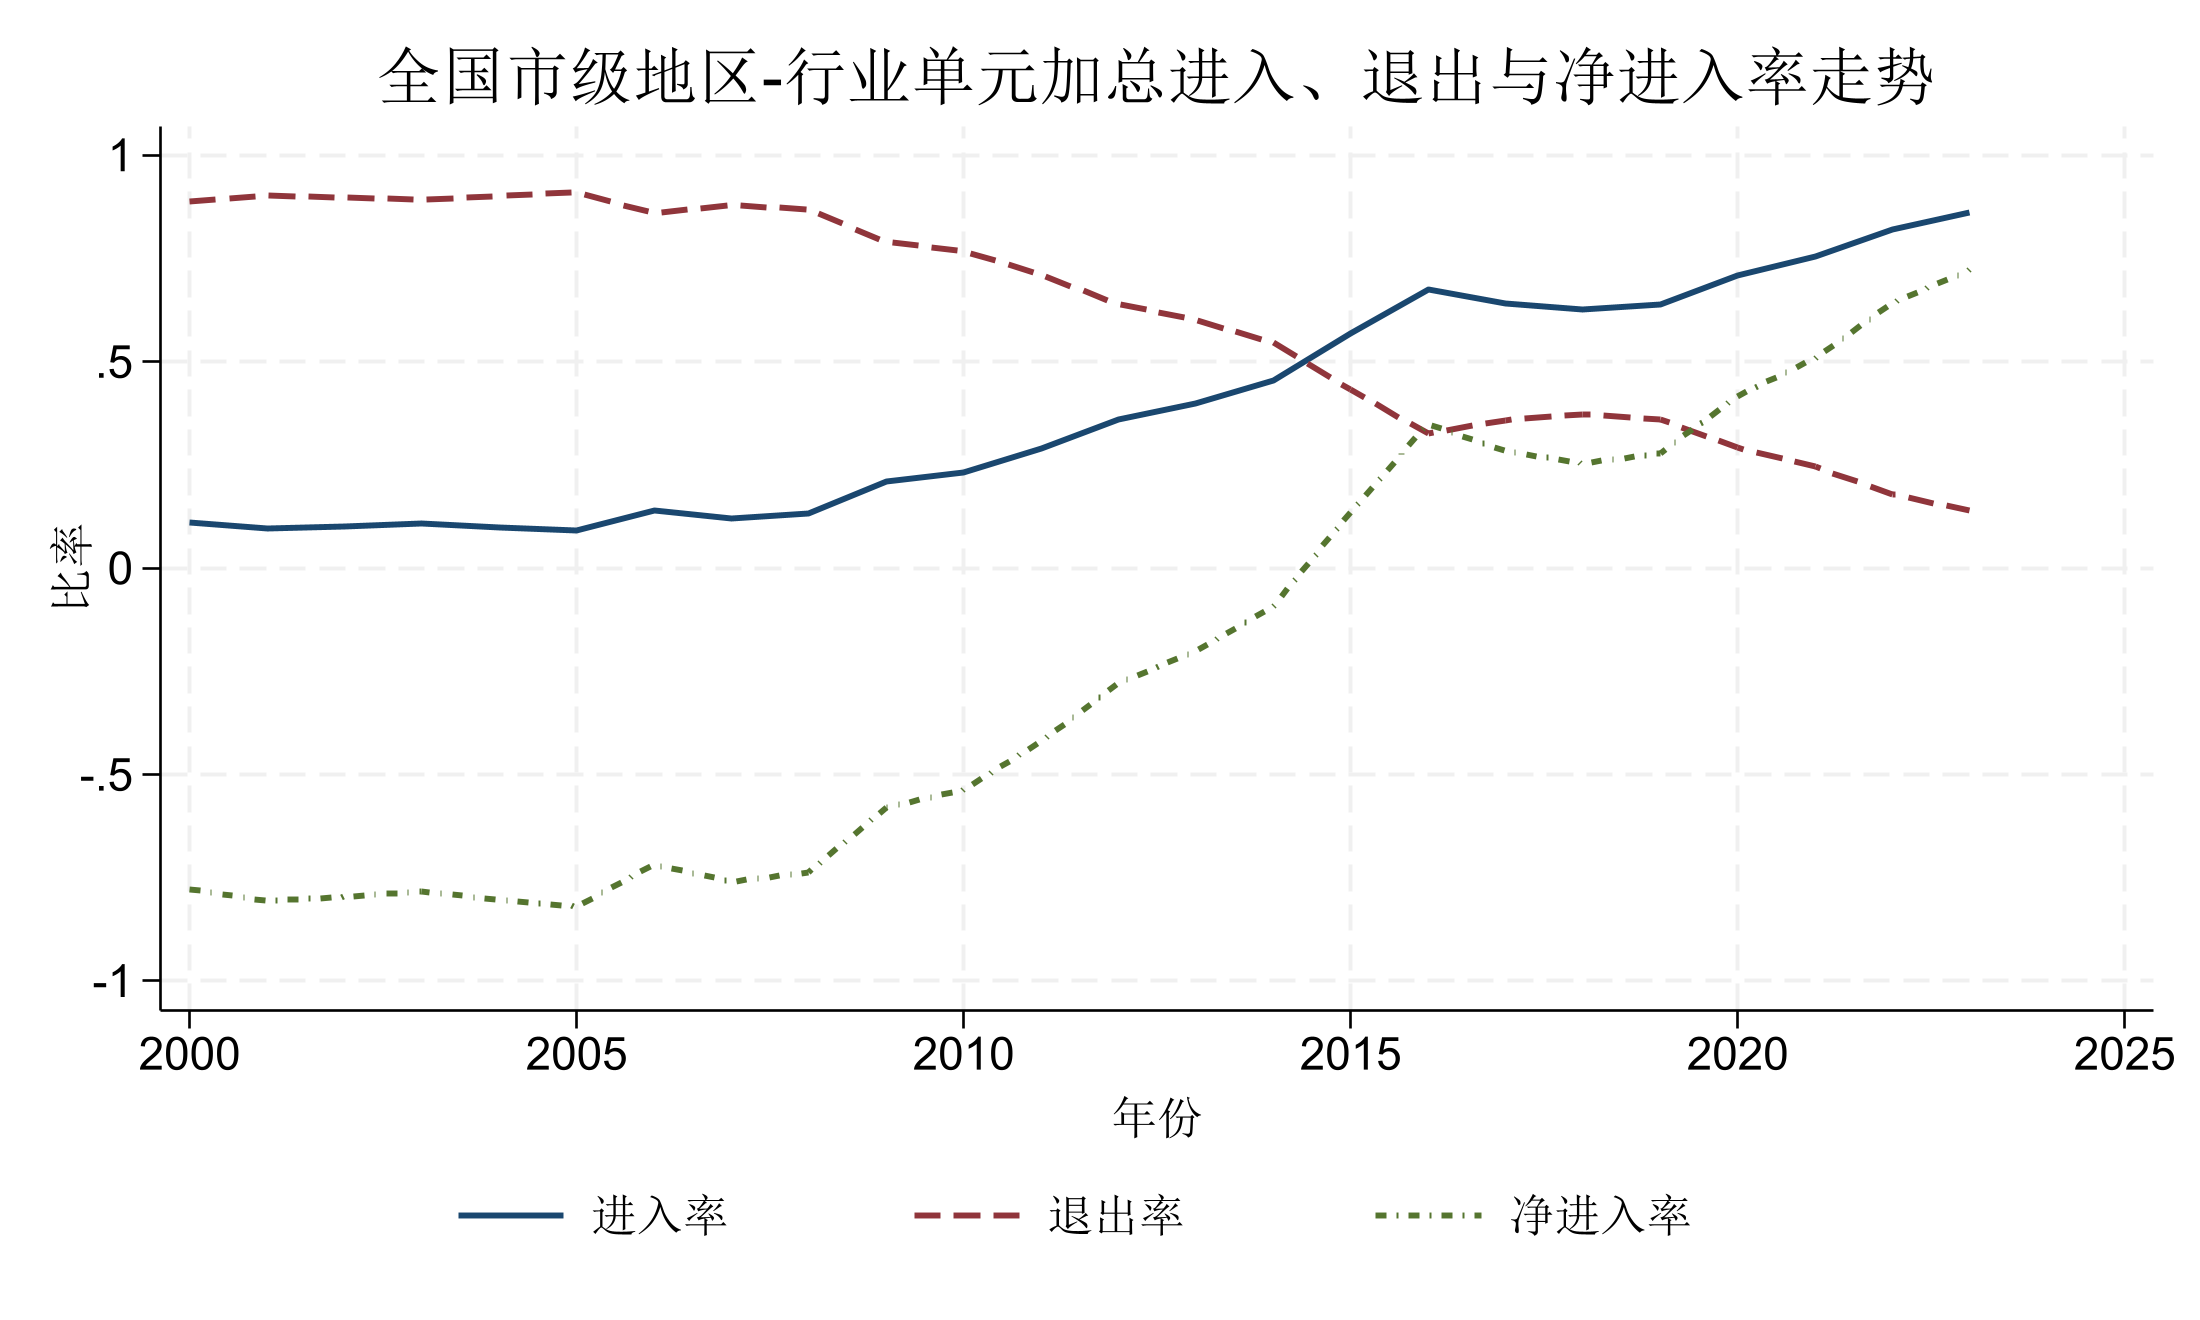
\includegraphics[width=0.9\textwidth]{../output/figures/figure1_national_index_trend.png}
\caption{全国市级地区--行业单元加总进入率、退出率与净进入率走势}
\caption*{\footnotesize 注：横轴为年份，纵轴为按全国市级地区--行业单元加总后的比率。蓝色实线表示进入率，红色虚线表示退出率，绿色点划线表示净进入率，三条线共同反映全国总体企业动态的时间变化。}
\end{figure}

\begin{figure}[H]
\centering
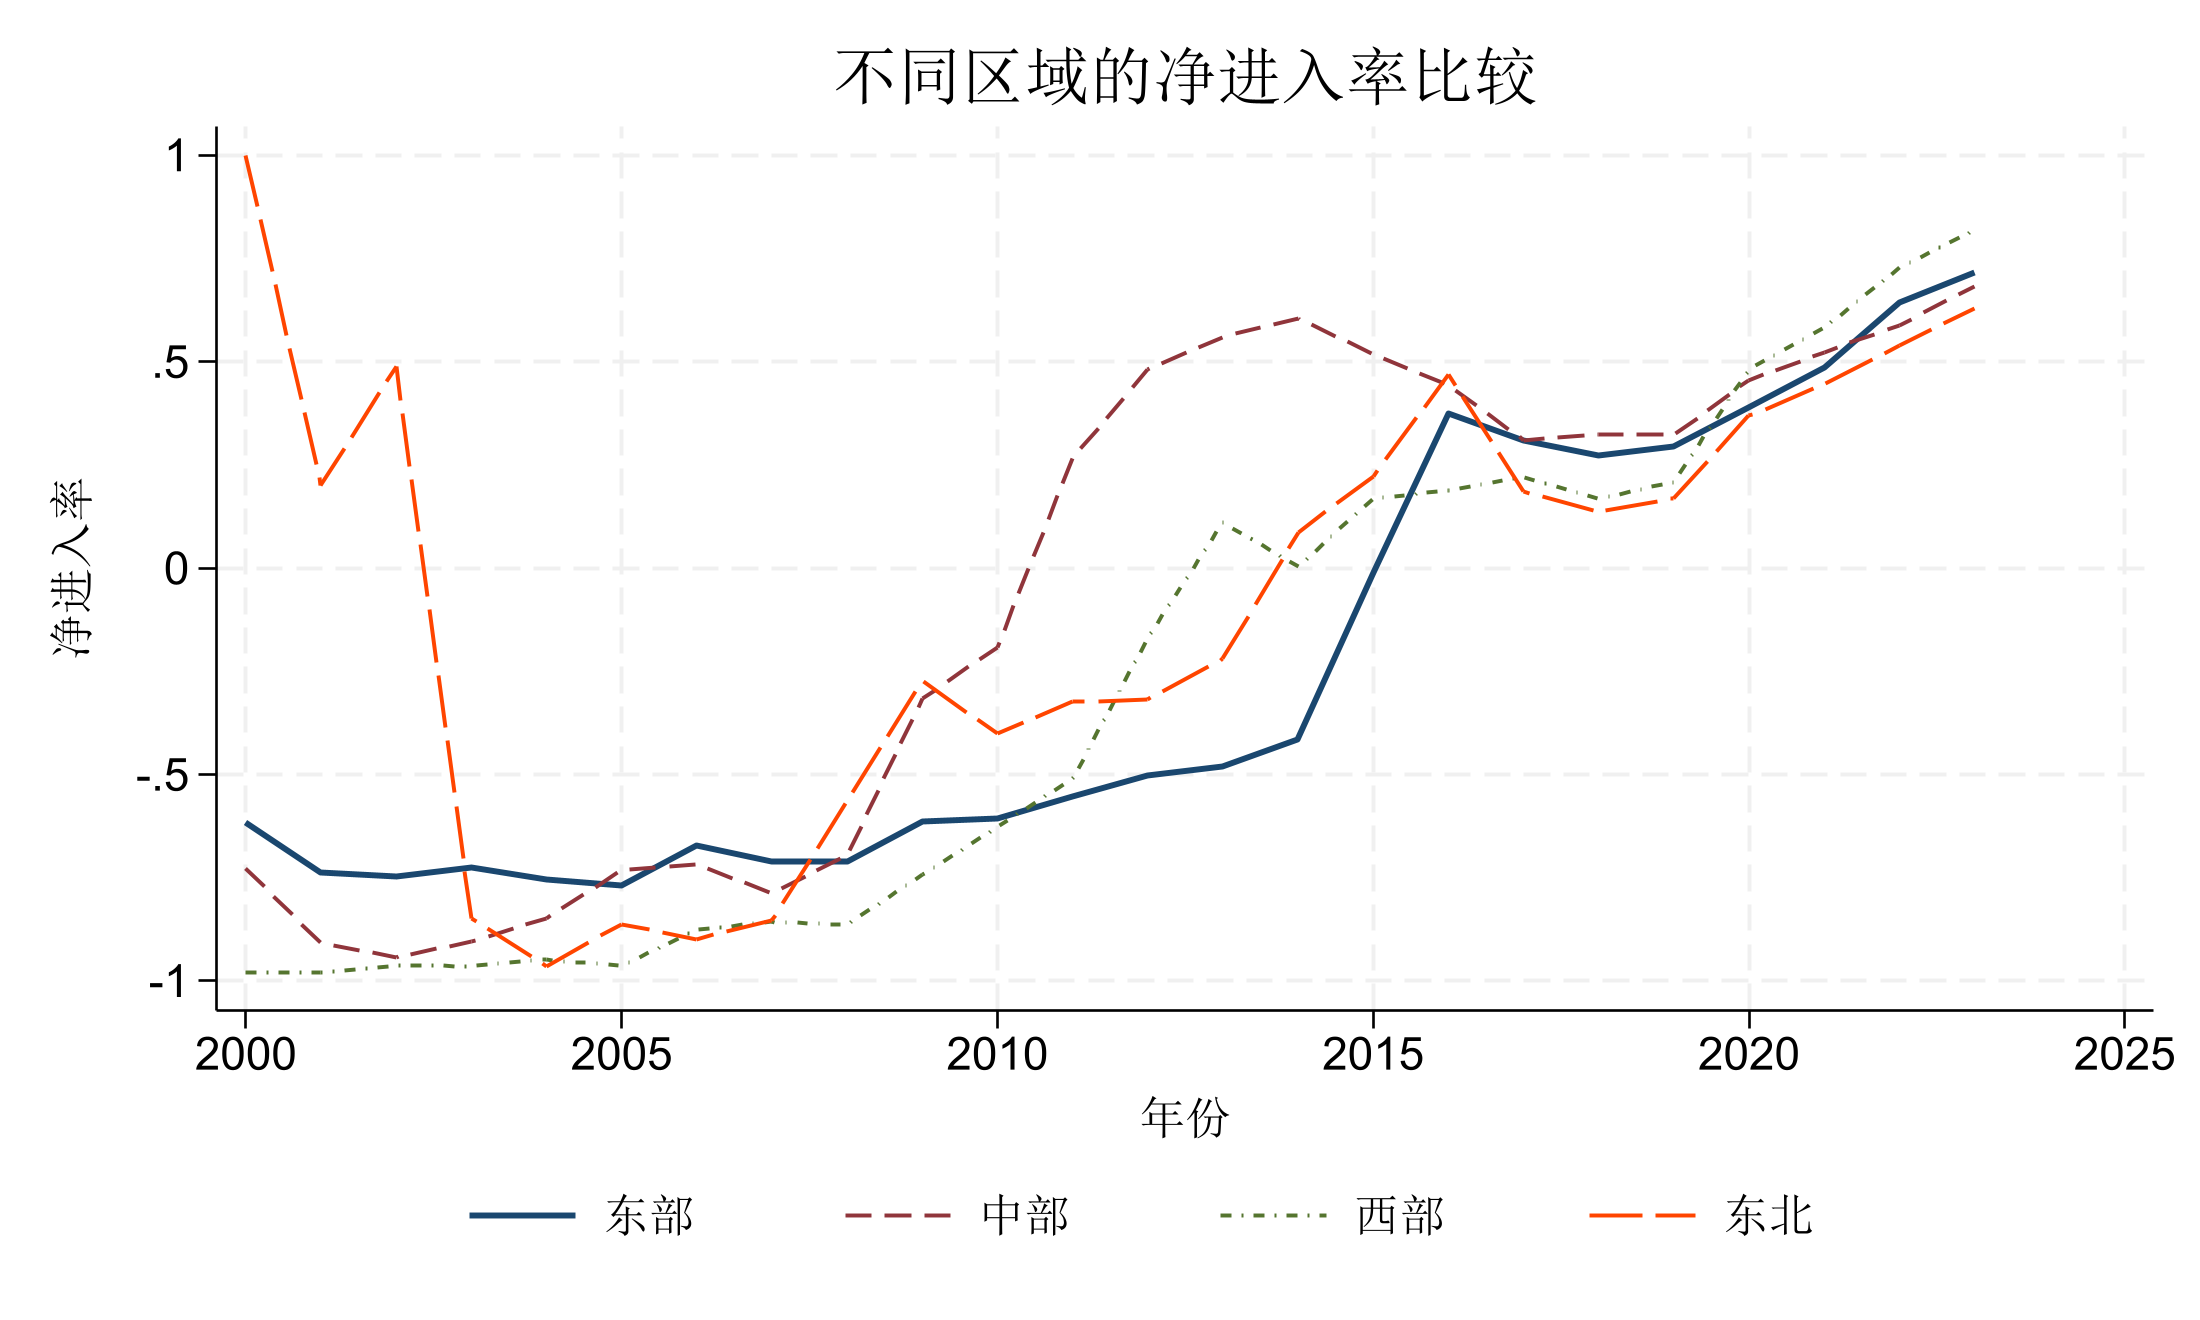
\includegraphics[width=0.9\textwidth]{../output/figures/figure2_region_comparison.png}
\caption{不同区域净进入率比较}
\caption*{\footnotesize 注：横轴为年份，纵轴为区域净进入率。不同颜色的折线分别对应东部、中部、西部和东北地区，用于比较四大区域企业净进入表现的长期差异。}
\end{figure}

为了把行业单元层面的信息回收至城市层面，本文将同一城市同一年内全部有效行业单元加总，得到城市年度进入率、退出率和净进入率。考虑到极端比率值在城市排序中可能带来误导，本文不再展示“净进入率前 20 城市”，而改用更稳健的城市平均进入率与退出率关系图以及排名变动图来刻画城市间差异。图 3 展示了城市平均进入率与平均退出率之间的对应关系。位于 45 度线之上的城市，其长期平均进入率高于退出率，也意味着具有更强的净进入表现；圆点越大，则说明该城市在样本中的聚合企业规模越大，因此图 3 同时呈现了城市表现与样本权重两层信息。

\begin{figure}[H]
\centering
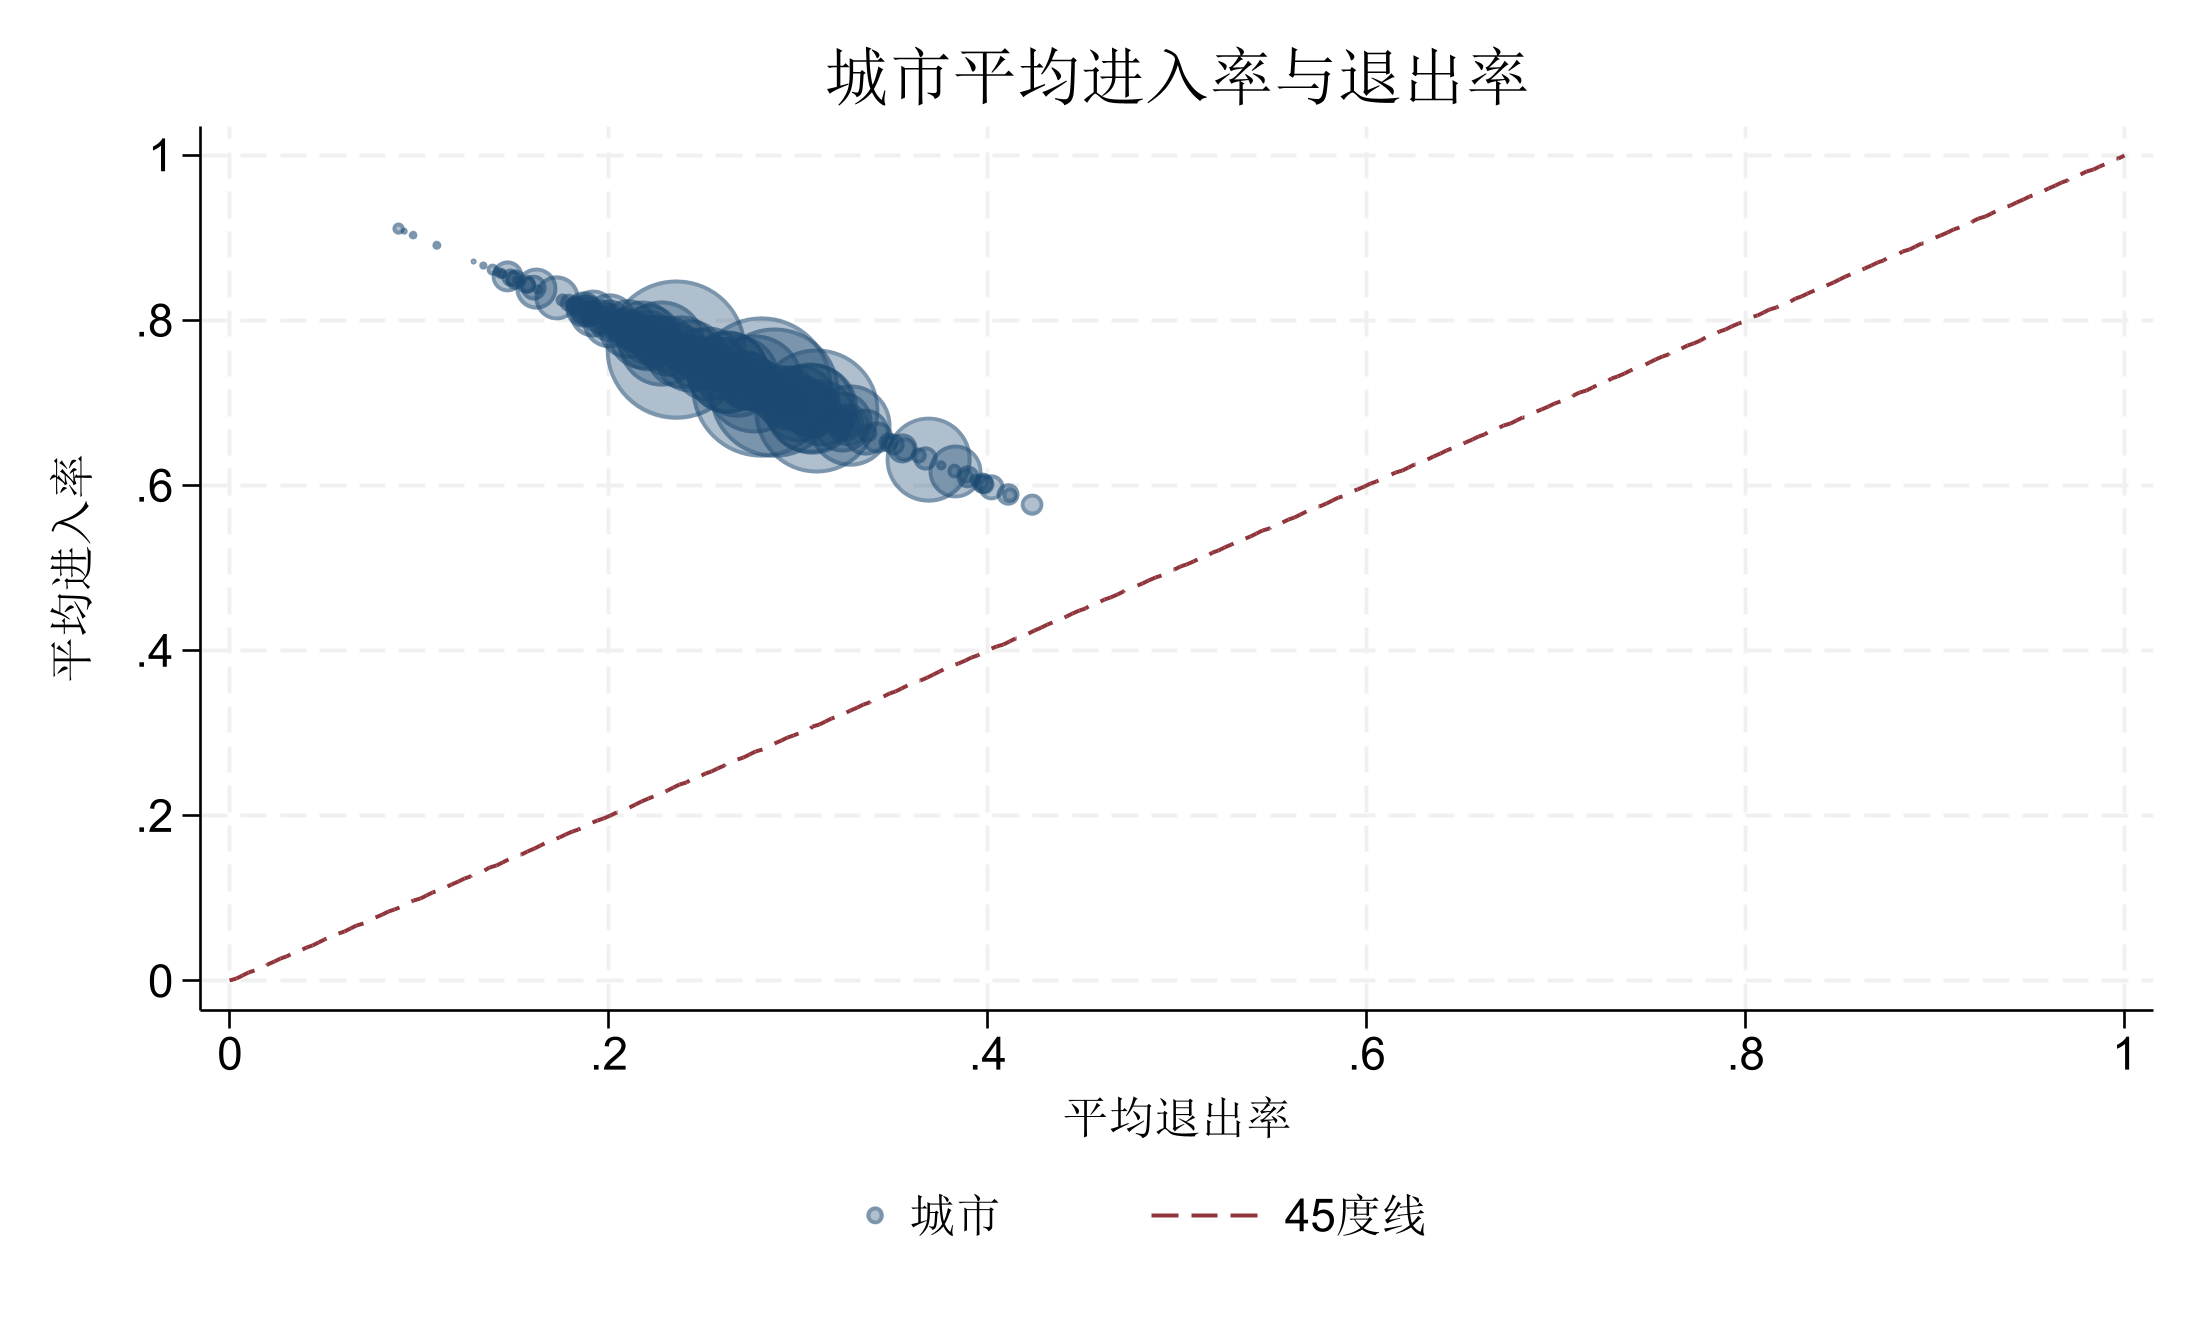
\includegraphics[width=0.8\textwidth]{../output/figures/figure3_entry_exit_scatter.png}
\caption{城市平均进入率与退出率}
\caption*{\footnotesize 注：横轴为城市在样本期内的平均退出率，纵轴为平均进入率。每个圆点代表一个城市，圆点大小按该城市聚合企业总数加权，因此圈子越大表示样本企业规模越大；45 度线表示进入率等于退出率，位于其上方的城市具有更高的平均净进入。}
\end{figure}

城市排序的动态变化同样值得关注。由于要求城市在相应年份具备足够多的有效行业单元和聚合企业规模，2000 年与 2023 年的共同样本较为严格，因此本文不再强调“排名提升最快的城市”，而是报告“排名变动最大的城市”。图 4 展示了 2000--2023 年净进入率排名变动绝对值最大的 15 个城市，图 6 则画出了北京、上海、广州、深圳、杭州和成都等代表性城市的长期排名轨迹，图 7 则展示了净进入率分布在 2000 年、2010 年和 2023 年的变化。将这三幅图放在一起看，可以更完整地理解城市间差异既体现在平均水平上，也体现在分布扩散与排名重排上。

与企业进入退出直接相关的另一条线索是产业结构变化。图 5 给出了城市产业集中度 HHI 的年度走势。可以看到，HHI 从 2000 年的较高水平持续下降，到 2020 年前后已明显低于样本初期，2023 年略有回升但整体仍处于较低位置。这意味着随着城市有效行业单元的大幅扩张，城市产业结构整体趋于多元化，而不是越来越集中于少数行业。由此，前文观察到的持续净进入，并不是在更狭窄的产业空间内完成的，而是在\textbf{更分散、更多元的城市产业结构}中实现的。

\begin{figure}[H]
\centering
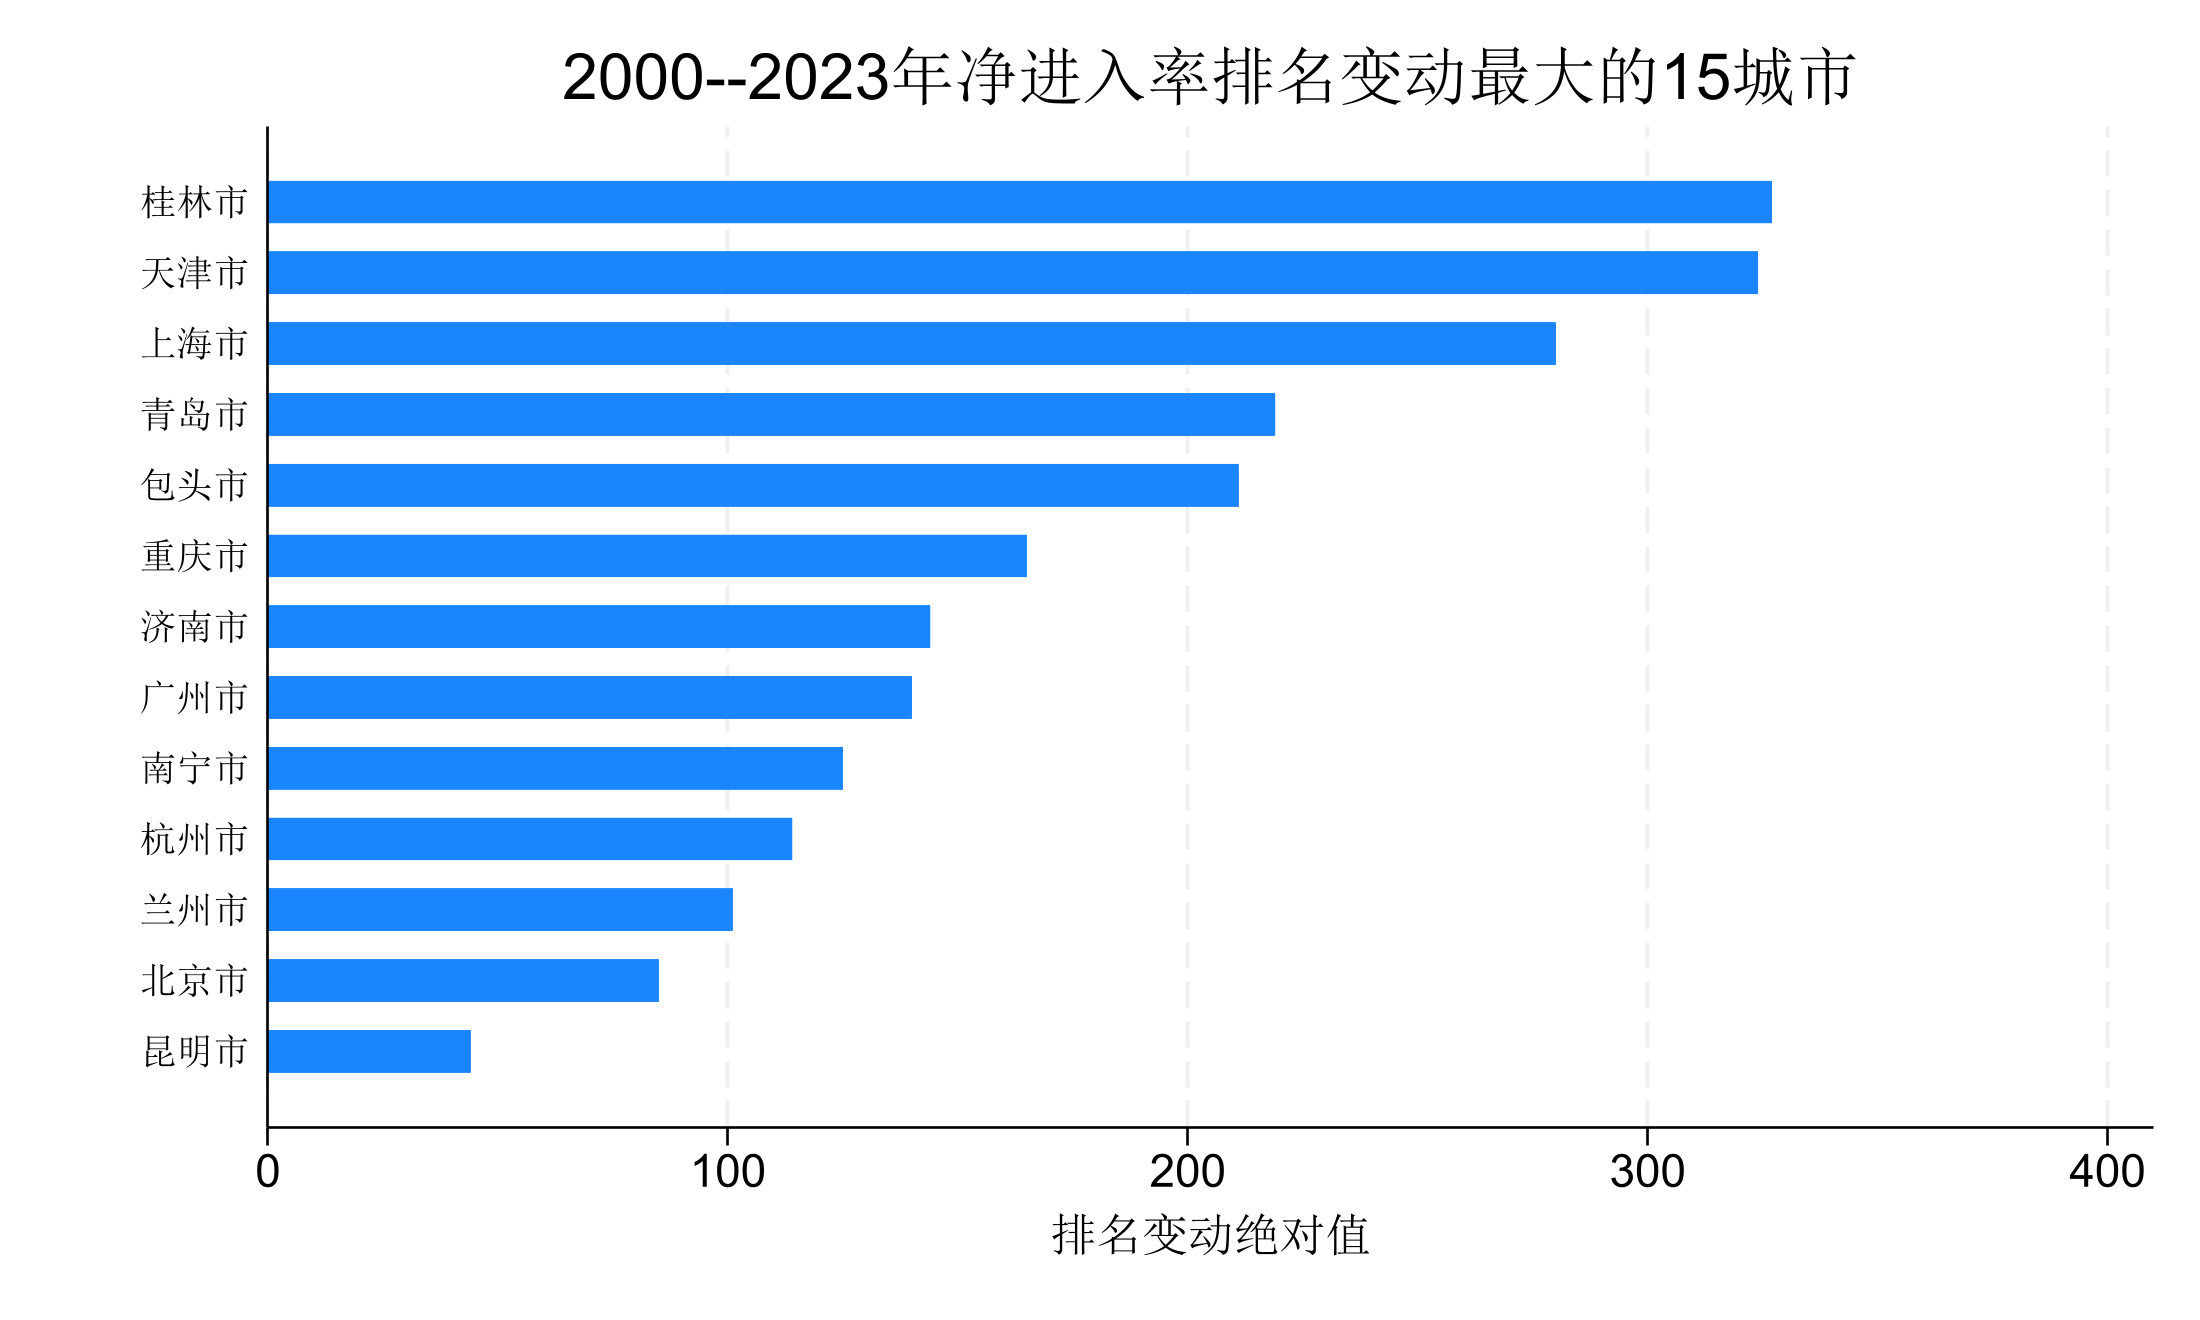
\includegraphics[width=0.9\textwidth]{../output/figures/figure4_rank_improvers.png}
\caption{2000--2023 年净进入率排名变动最大的 15 城市}
\caption*{\footnotesize 注：横轴无实际数值含义，纵轴为城市名称。柱长表示城市在 2000 年和 2023 年之间净进入率排名变动的绝对值，数值越大表示名次变化越剧烈。}
\end{figure}

\begin{figure}[H]
\centering
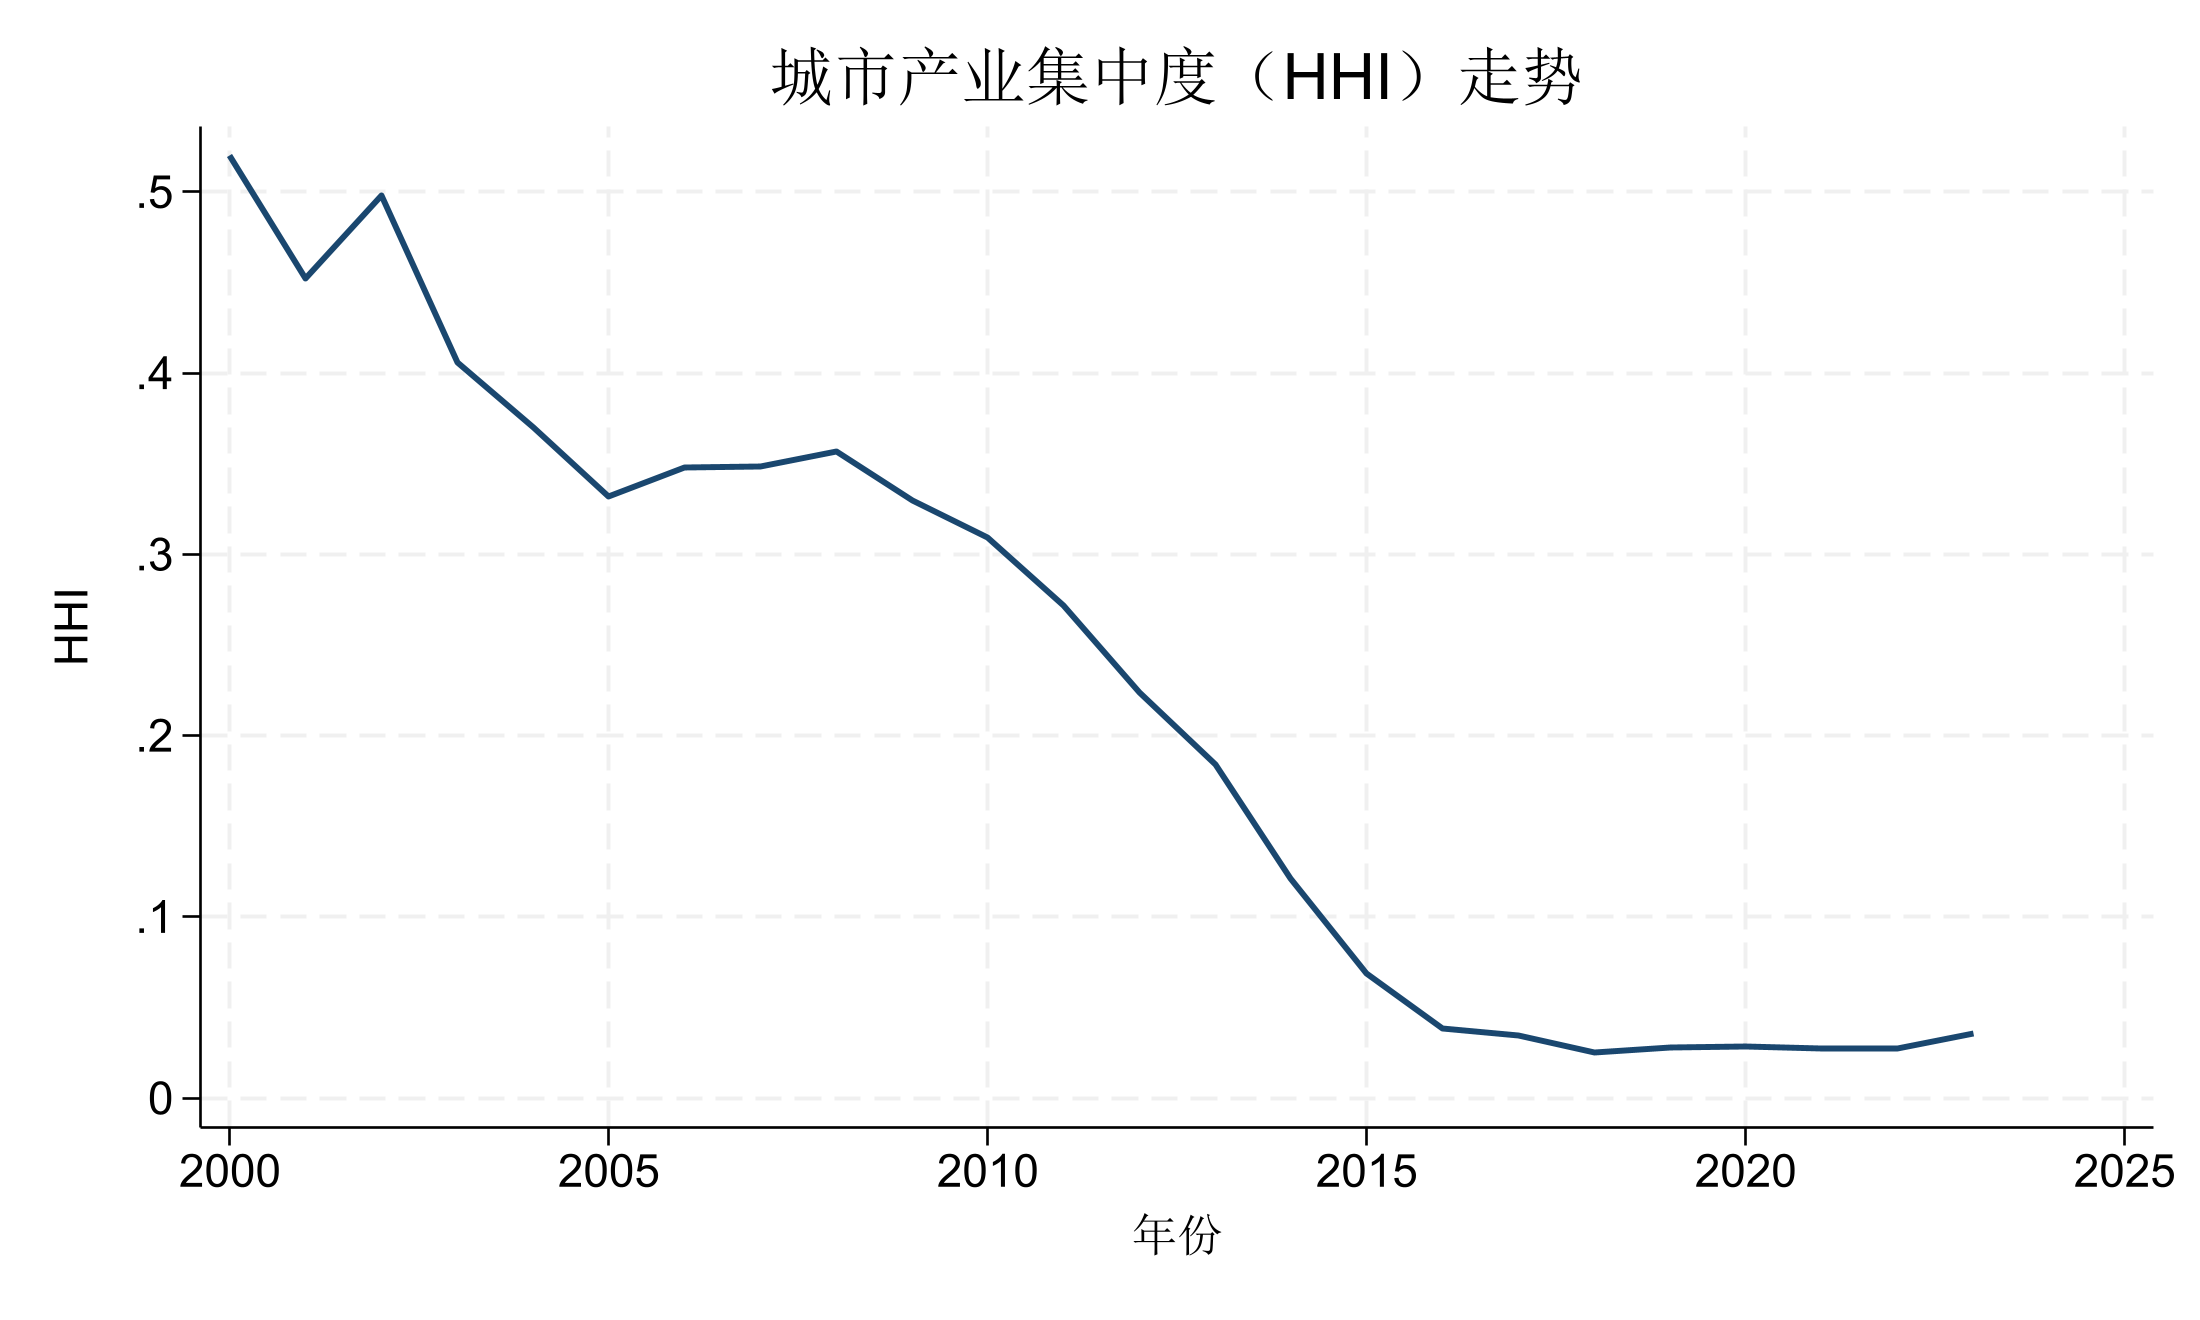
\includegraphics[width=0.82\textwidth]{../output/figures/figure5_hhi_trend.png}
\caption{城市产业集中度（HHI）走势}
\caption*{\footnotesize 注：横轴为年份，纵轴为城市--年份层面平均 HHI。折线越高表示城市产业更集中于少数行业，越低表示行业结构更分散、更多元。}
\end{figure}

\begin{figure}[H]
\centering
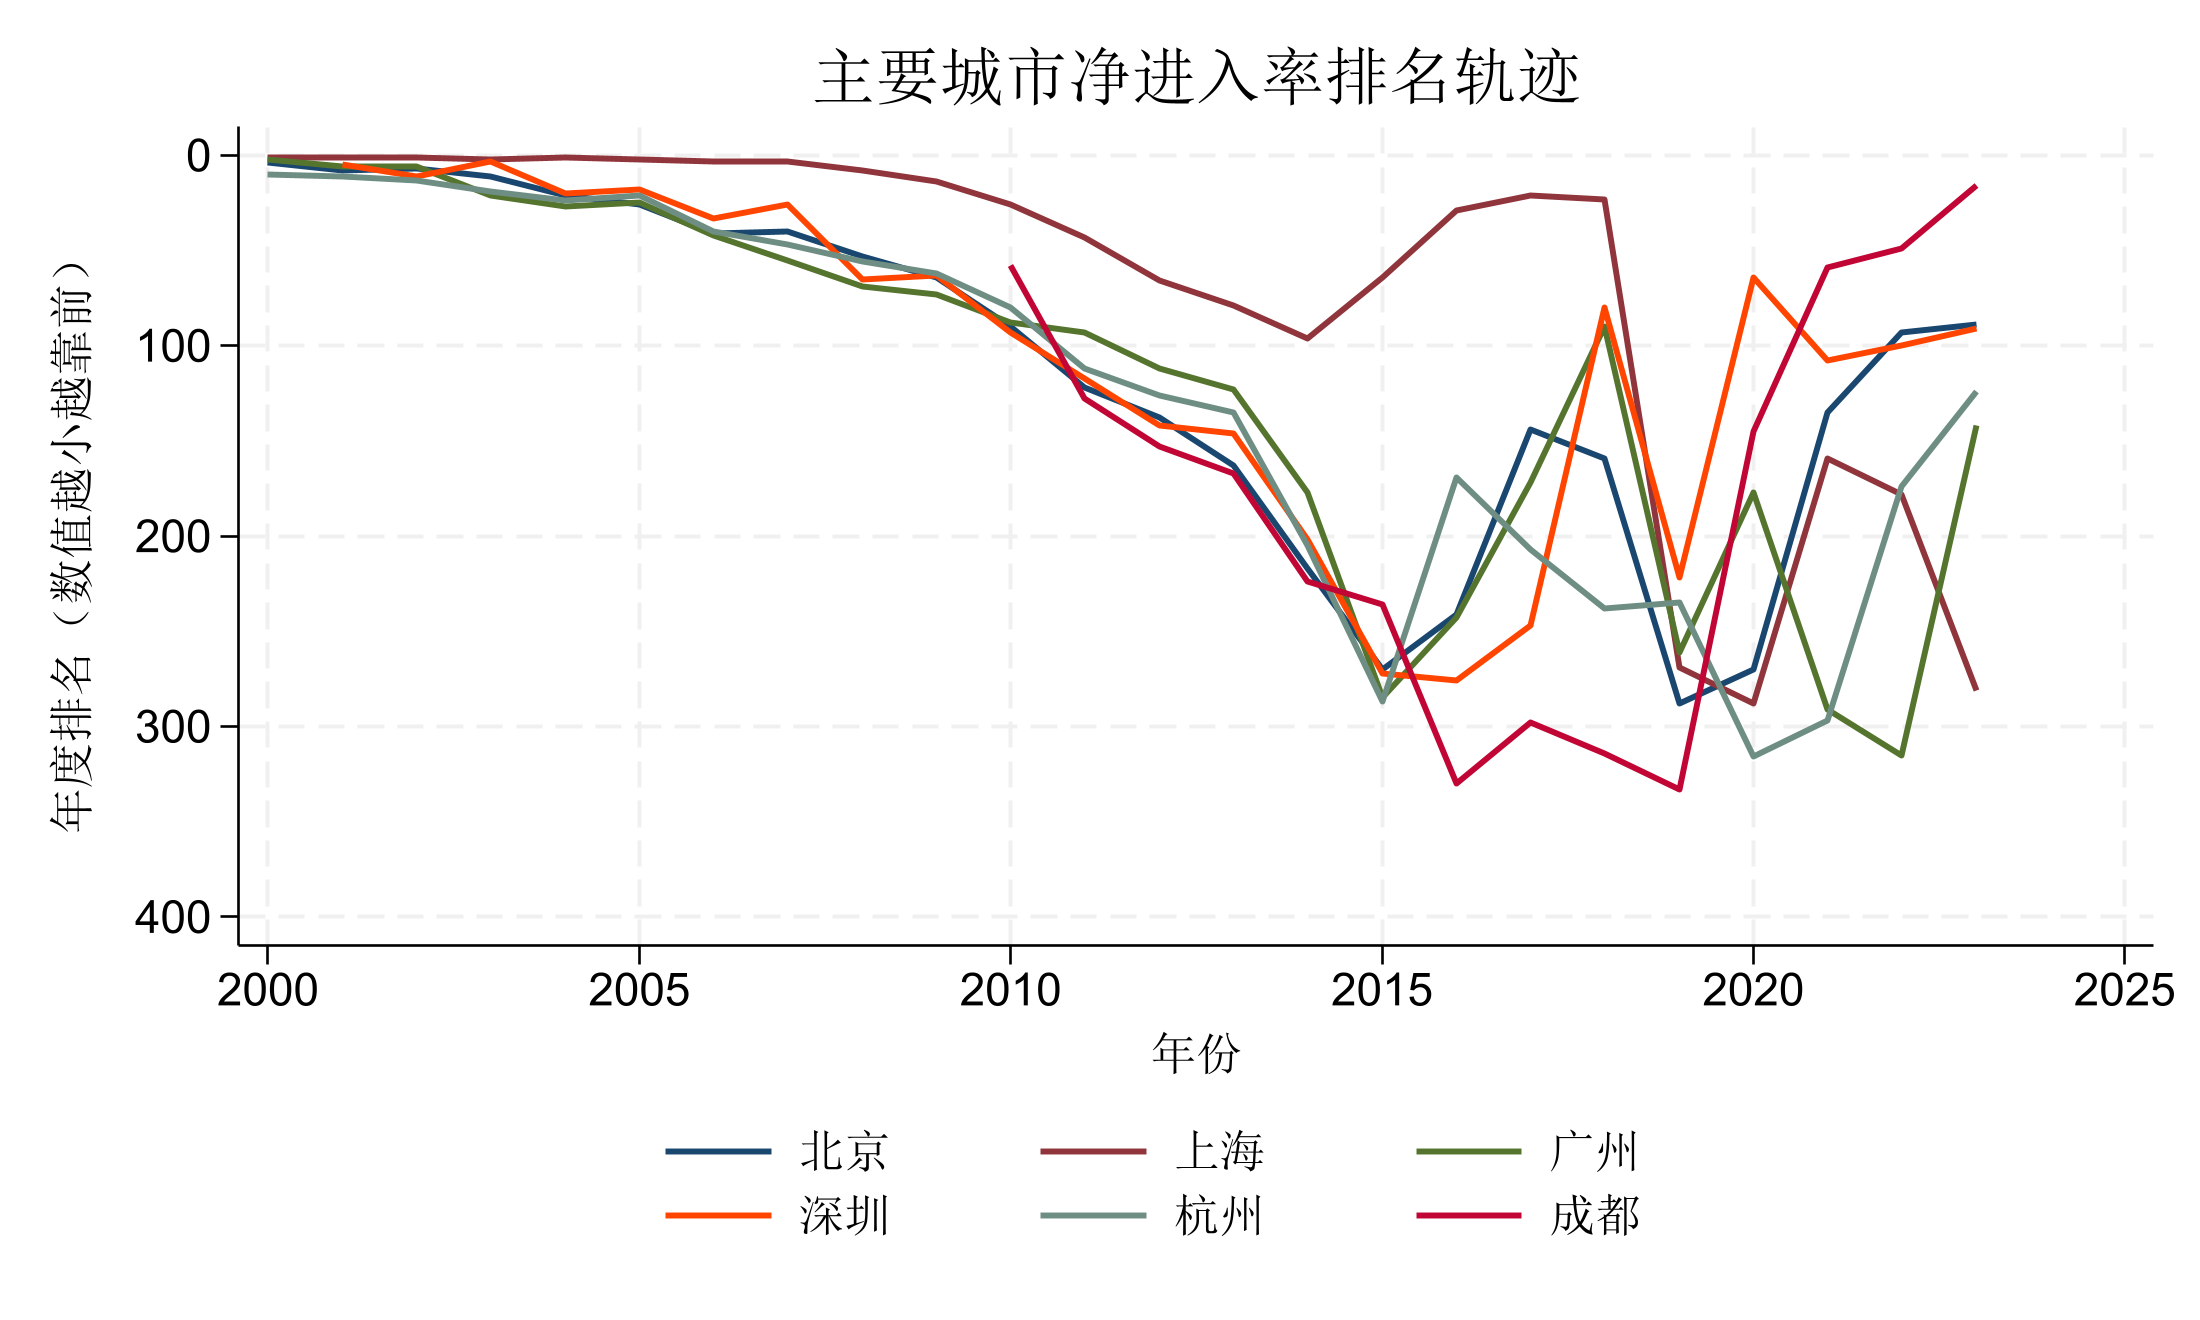
\includegraphics[width=0.9\textwidth]{../output/figures/figure6_topcity_rank_paths.png}
\caption{主要城市净进入率排名轨迹}
\caption*{\footnotesize 注：横轴为年份，纵轴为年度排名，数值越小表示排名越靠前。不同颜色折线分别代表北京、上海、广州、深圳、杭州和成都，用于比较头部城市净进入率相对位置的动态变化。}
\end{figure}

\begin{figure}[H]
\centering
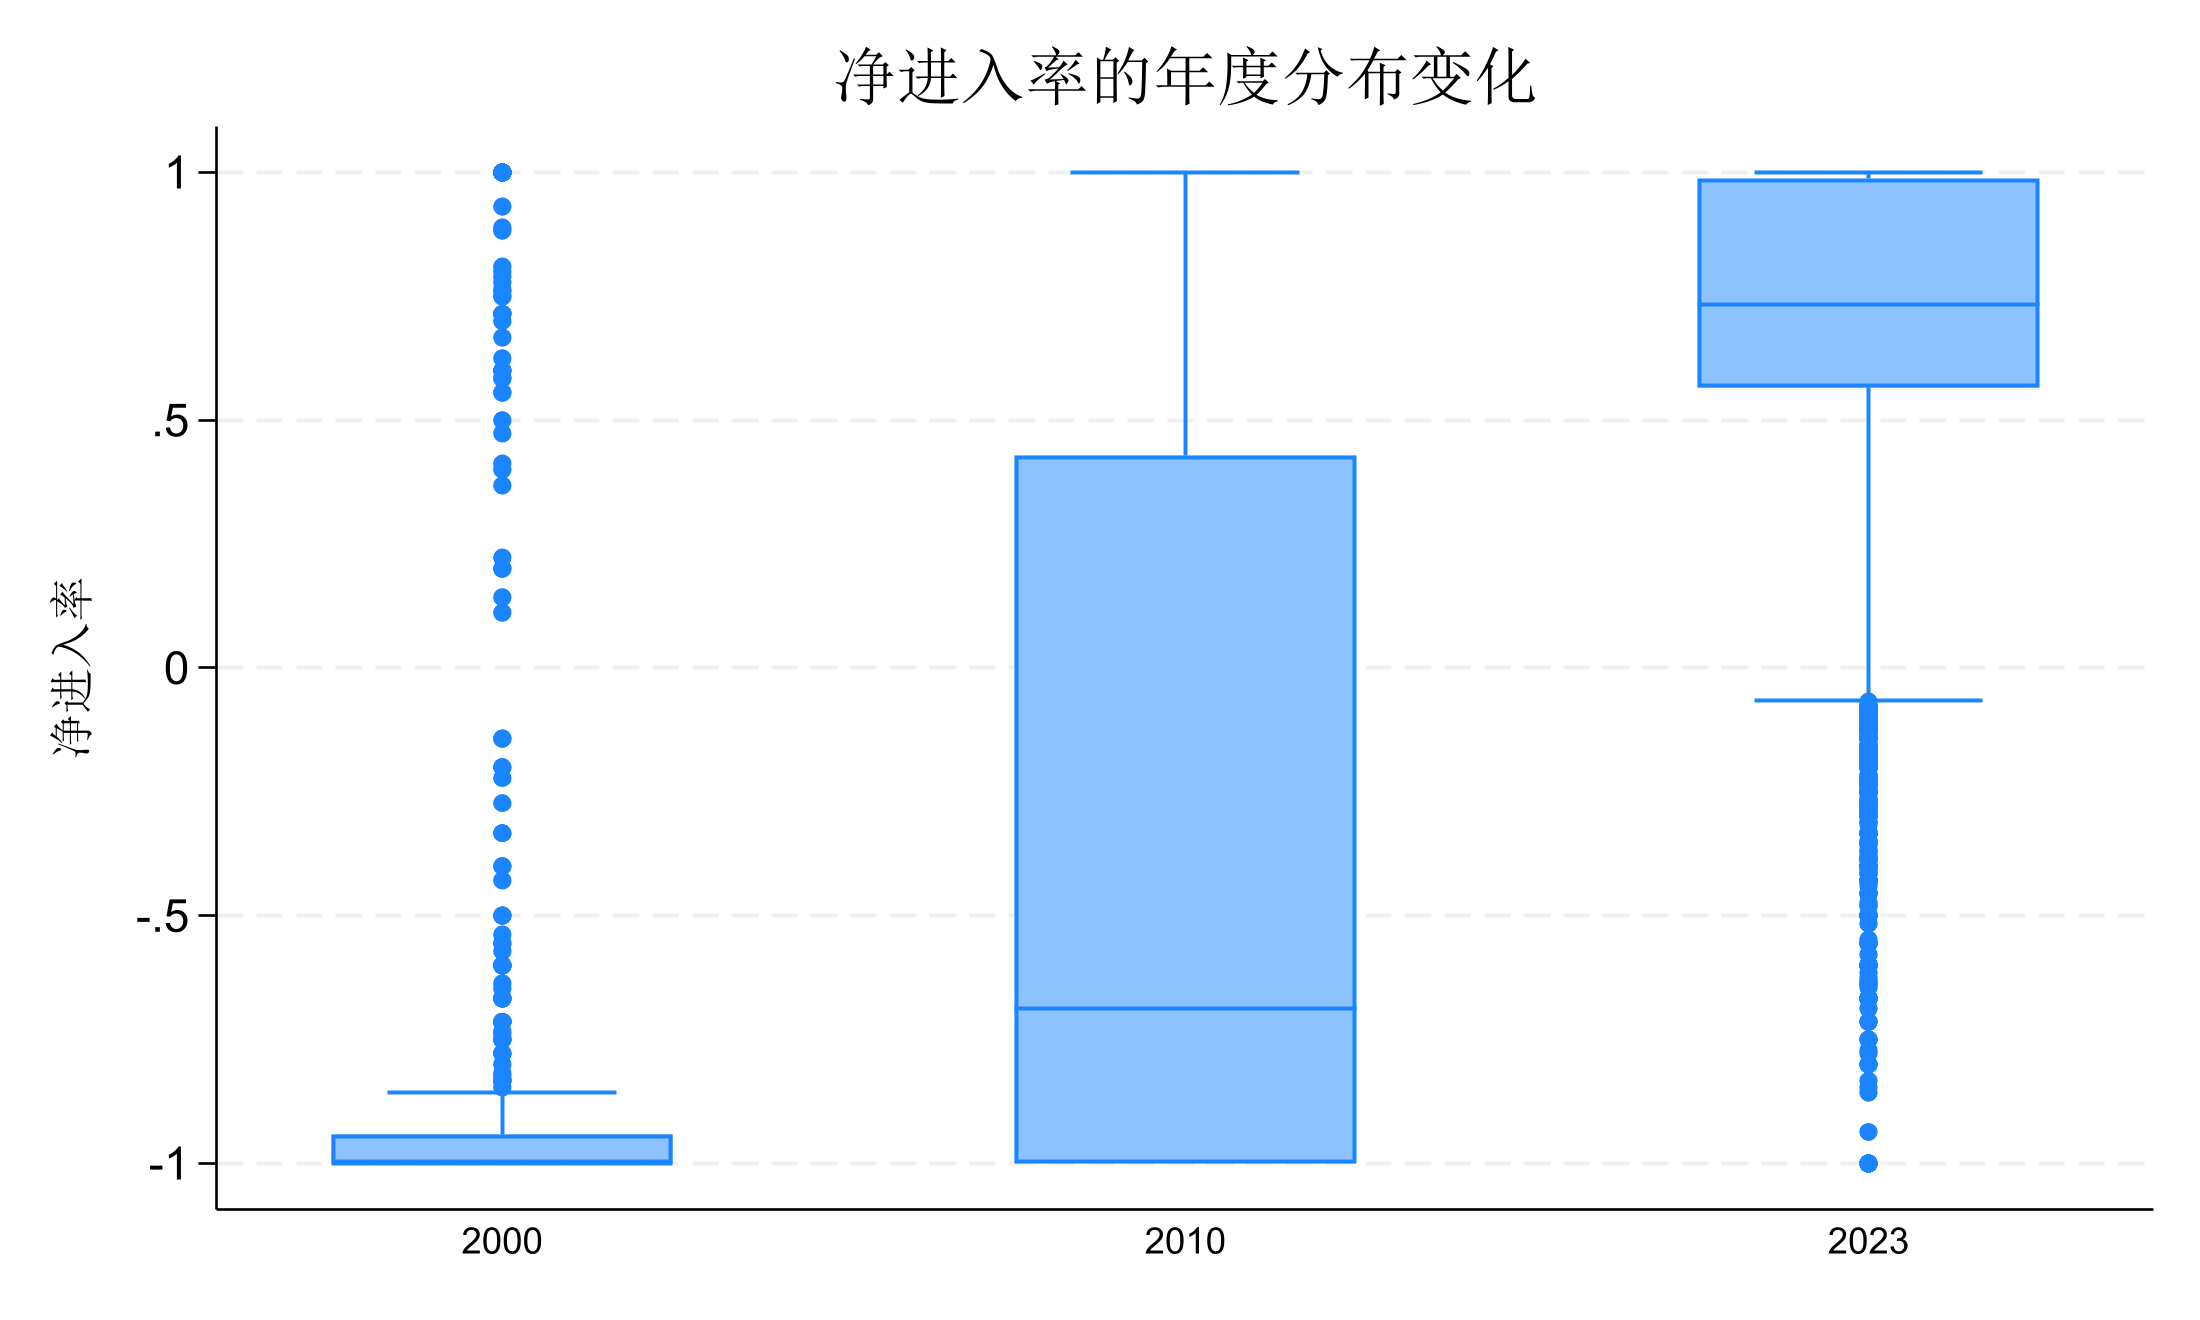
\includegraphics[width=0.8\textwidth]{../output/figures/figure7_index_distribution_box.png}
\caption{净进入率的年度分布变化}
\caption*{\footnotesize 注：横轴为年份组别，纵轴为净进入率。箱体表示四分位区间，中位线表示中位数，须线反映非异常值范围，用于比较不同时点行业单元净进入率分布的离散程度。}
\end{figure}

\section{面板回归结果}
在统一的市级地区--行业--年份口径下，本文进一步估计固定效应模型。基准回归的被解释变量分别为净进入率、进入率和退出率，核心解释变量为滞后一期单元企业数对数，并加入相应指标的滞后项以及滞后一期城市产业集中度 HHI。固定效应设定为城市--行业固定效应，并在主要模型中加入年份固定效应，标准误聚类到城市层面。由于滞后项的引入，最终进入回归的有效样本为 395,593 个城市--行业--年份观测。这里的经验策略并不追求因果识别，而是希望回答一个更基础的问题：在控制了单元不随时间变化的特征以及年度共同冲击之后，行业单元规模、产业结构与进入退出之间是否仍存在稳定的条件相关关系。

\begin{table}[htbp]\centering
\def\sym#1{\ifmmode^{#1}\else\(^{#1}\)\fi}
\caption{市级地区-行业-年份样本：基准固定效应回归}
\begin{tabular}{l*{4}{c}}
\toprule
                    &\multicolumn{1}{c}{(1)}&\multicolumn{1}{c}{(2)}&\multicolumn{1}{c}{(3)}&\multicolumn{1}{c}{(4)}\\
                    &\multicolumn{1}{c}{净进入率}&\multicolumn{1}{c}{净进入率}&\multicolumn{1}{c}{进入率}&\multicolumn{1}{c}{退出率}\\
\midrule
滞后一期单元企业数对数&       0.146\sym{***}&     -0.0103\sym{**} &    -0.00515\sym{**} &     0.00515\sym{**} \\
                    &    (0.0113)         &   (0.00442)         &   (0.00221)         &   (0.00221)         \\
\addlinespace
滞后一期净进入率    &                     &       0.449\sym{***}&                     &                     \\
                    &                     &    (0.0117)         &                     &                     \\
\addlinespace
滞后一期城市行业集中度HHI&                     &      0.0997         &      0.0498         &     -0.0498         \\
                    &                     &     (0.103)         &    (0.0514)         &    (0.0514)         \\
\addlinespace
滞后一期进入率      &                     &                     &       0.449\sym{***}&                     \\
                    &                     &                     &    (0.0117)         &                     \\
\addlinespace
滞后一期退出率      &                     &                     &                     &       0.449\sym{***}\\
                    &                     &                     &                     &    (0.0117)         \\
\addlinespace
Constant            &      -0.128\sym{***}&      -0.397\sym{***}&      0.0767\sym{***}&       0.474\sym{***}\\
                    &    (0.0387)         &    (0.0566)         &    (0.0260)         &    (0.0315)         \\
\midrule
City-Industry FE    &         Yes         &         Yes         &         Yes         &         Yes         \\
Year FE             &          No         &         Yes         &         Yes         &         Yes         \\
Observations        &     395,593         &     395,593         &     395,593         &     395,593         \\
Within R-squared    &                     &                     &                     &                     \\
\bottomrule
\multicolumn{5}{l}{\footnotesize Standard errors in parentheses}\\
\multicolumn{5}{l}{\footnotesize \sym{*} \(p<0.10\), \sym{**} \(p<0.05\), \sym{***} \(p<0.01\)}\\
\end{tabular}
\end{table}


基准结果表明，地区--行业单元的进入退出指标存在明显持续性。滞后一期净进入率、进入率和退出率的系数都显著为正，说明行业单元中的企业动态具有较强路径依赖。进一步地，在控制年份固定效应、滞后净进入率和 HHI 后，滞后一期单元企业数对数对净进入率的系数转为显著负值，说明在同一城市--行业单元内部，更大的基期规模并不一定对应更高的后续净进入率，反而可能反映成熟行业进入边际趋缓。换言之，\textbf{规模扩张与持续净扩张并不是同一件事。}HHI 的估计系数为正，但在基准回归中并未达到常规显著性水平，这意味着产业集中度与企业动态之间的关系更可能依赖于城市类型或区域差异，而非简单的线性平均效应。

异质性回归进一步考察区域和城市等级差异。表 3 显示，东部地区的交互项显著为正，说明在东部城市中，行业单元规模与净进入率之间的负相关关系更弱，甚至部分被抵消。副省级城市的交互项也呈现正向且边际显著，这表明在行政等级更高、资源集聚更强的城市中，较大的行业单元更容易维持持续净进入。相比之下，省会城市的交互项方向为正但统计上不显著。滞后一期 HHI 在三组异质性回归中依旧没有表现出显著线性效应，这与基准结果基本一致。综合来看，企业动态的差异更多来自\textbf{城市发展阶段、区位条件与资源集聚能力}，而不是由单一的集中度指标直接决定。

\begin{table}[htbp]\centering
\def\sym#1{\ifmmode^{#1}\else\(^{#1}\)\fi}
\caption{市级地区-年份样本：异质性分析}
\begin{tabular}{l*{3}{c}}
\toprule
                    &\multicolumn{1}{c}{(1)}&\multicolumn{1}{c}{(2)}&\multicolumn{1}{c}{(3)}\\
                    &\multicolumn{1}{c}{净进入率}&\multicolumn{1}{c}{净进入率}&\multicolumn{1}{c}{退出率}\\
\midrule
滞后一期样本企业总数对数&      -0.123\sym{***}&     -0.0278\sym{***}&      0.0142\sym{***}\\
                    &    (0.0168)         &   (0.00506)         &   (0.00251)         \\
\addlinespace
east=0              &           0         &                     &                     \\
                    &         (.)         &                     &                     \\
\addlinespace
east=1              &           0         &                     &                     \\
                    &         (.)         &                     &                     \\
\addlinespace
east=0 $\times$ 滞后一期样本企业总数对数&           0         &                     &                     \\
                    &         (.)         &                     &                     \\
\addlinespace
east=1 $\times$ 滞后一期样本企业总数对数&     -0.0383\sym{***}&                     &                     \\
                    &   (0.00805)         &                     &                     \\
\addlinespace
滞后一期进入率      &                     &       1.449\sym{***}&                     \\
                    &                     &    (0.0535)         &                     \\
\addlinespace
省会城市=0          &                     &           0         &                     \\
                    &                     &         (.)         &                     \\
\addlinespace
省会城市=1          &                     &           0         &                     \\
                    &                     &         (.)         &                     \\
\addlinespace
省会城市=0 $\times$ 滞后一期进入率&                     &           0         &                     \\
                    &                     &         (.)         &                     \\
\addlinespace
省会城市=1 $\times$ 滞后一期进入率&                     &       0.157\sym{***}&                     \\
                    &                     &    (0.0404)         &                     \\
\addlinespace
滞后一期退出率      &                     &                     &       0.729\sym{***}\\
                    &                     &                     &    (0.0262)         \\
\addlinespace
副省级城市=0        &                     &                     &           0         \\
                    &                     &                     &         (.)         \\
\addlinespace
副省级城市=1        &                     &                     &           0         \\
                    &                     &                     &         (.)         \\
\addlinespace
副省级城市=0 $\times$ 滞后一期退出率&                     &                     &           0         \\
                    &                     &                     &         (.)         \\
\addlinespace
副省级城市=1 $\times$ 滞后一期退出率&                     &                     &      0.0733\sym{***}\\
                    &                     &                     &    (0.0209)         \\
\addlinespace
Constant            &       1.087\sym{***}&      -0.477\sym{***}&     0.00592         \\
                    &    (0.0846)         &    (0.0479)         &    (0.0133)         \\
\midrule
City FE             &         Yes         &         Yes         &         Yes         \\
Year FE             &         Yes         &         Yes         &         Yes         \\
Observations        &       7,856         &       7,856         &       7,856         \\
Within R-squared    &                     &                     &                     \\
\bottomrule
\multicolumn{4}{l}{\footnotesize Standard errors in parentheses}\\
\multicolumn{4}{l}{\footnotesize \sym{*} \(p<0.10\), \sym{**} \(p<0.05\), \sym{***} \(p<0.01\)}\\
\end{tabular}
\end{table}


\section{行业结构与城市营商活力}
既然主样本本身就是行业维度面板，行业异质性就不是附属问题，而是本文主线的一部分。为此，本文将样本期内各行业的进入率、退出率、净进入率和样本企业规模进一步汇总。结果显示，样本规模最大的行业主要集中在批发、软件、技术服务、建筑装修和综合管理服务等领域。这些行业不仅吸纳了大量企业进入，而且在多数城市中也是企业动态最活跃的行业板块。也就是说，城市营商活力并不是均匀分布在所有行业中的，而是表现出明显的行业集中承载特征。

图 8 展示了样本规模最大的 15 个行业的平均净进入率。可以看到，不同行业之间的净进入表现差异明显。部分服务业和专业技术类行业呈现更高的平均净进入率，说明其新企业涌入更快、扩张更为显著；而一些传统批发或互联网相关行业虽然规模很大，但净进入率未必处于最高水平，说明\textbf{“大行业”并不必然意味着“最强的创业净扩张”。}

进一步地，图 9 和图 10 选取样本规模最大的四个行业，分别考察其进入率和退出率走势。整体上，这些行业在样本后期的比率波动更明显，既体现出创业活动更为活跃，也反映出竞争和市场出清同步加强。结合 HHI 的长期下降事实，可以推断中国城市营商活力的一个重要特征是：在产业结构不断多元化的同时，大行业仍持续主导着企业进入退出总量，但行业间的创业生态分化正在增强。由此，本文关于“营商活力”的理解并不是单一城市总量增长，而是\textbf{城市内部行业生态的差异化扩张与重组。}

\begin{figure}[H]
\centering
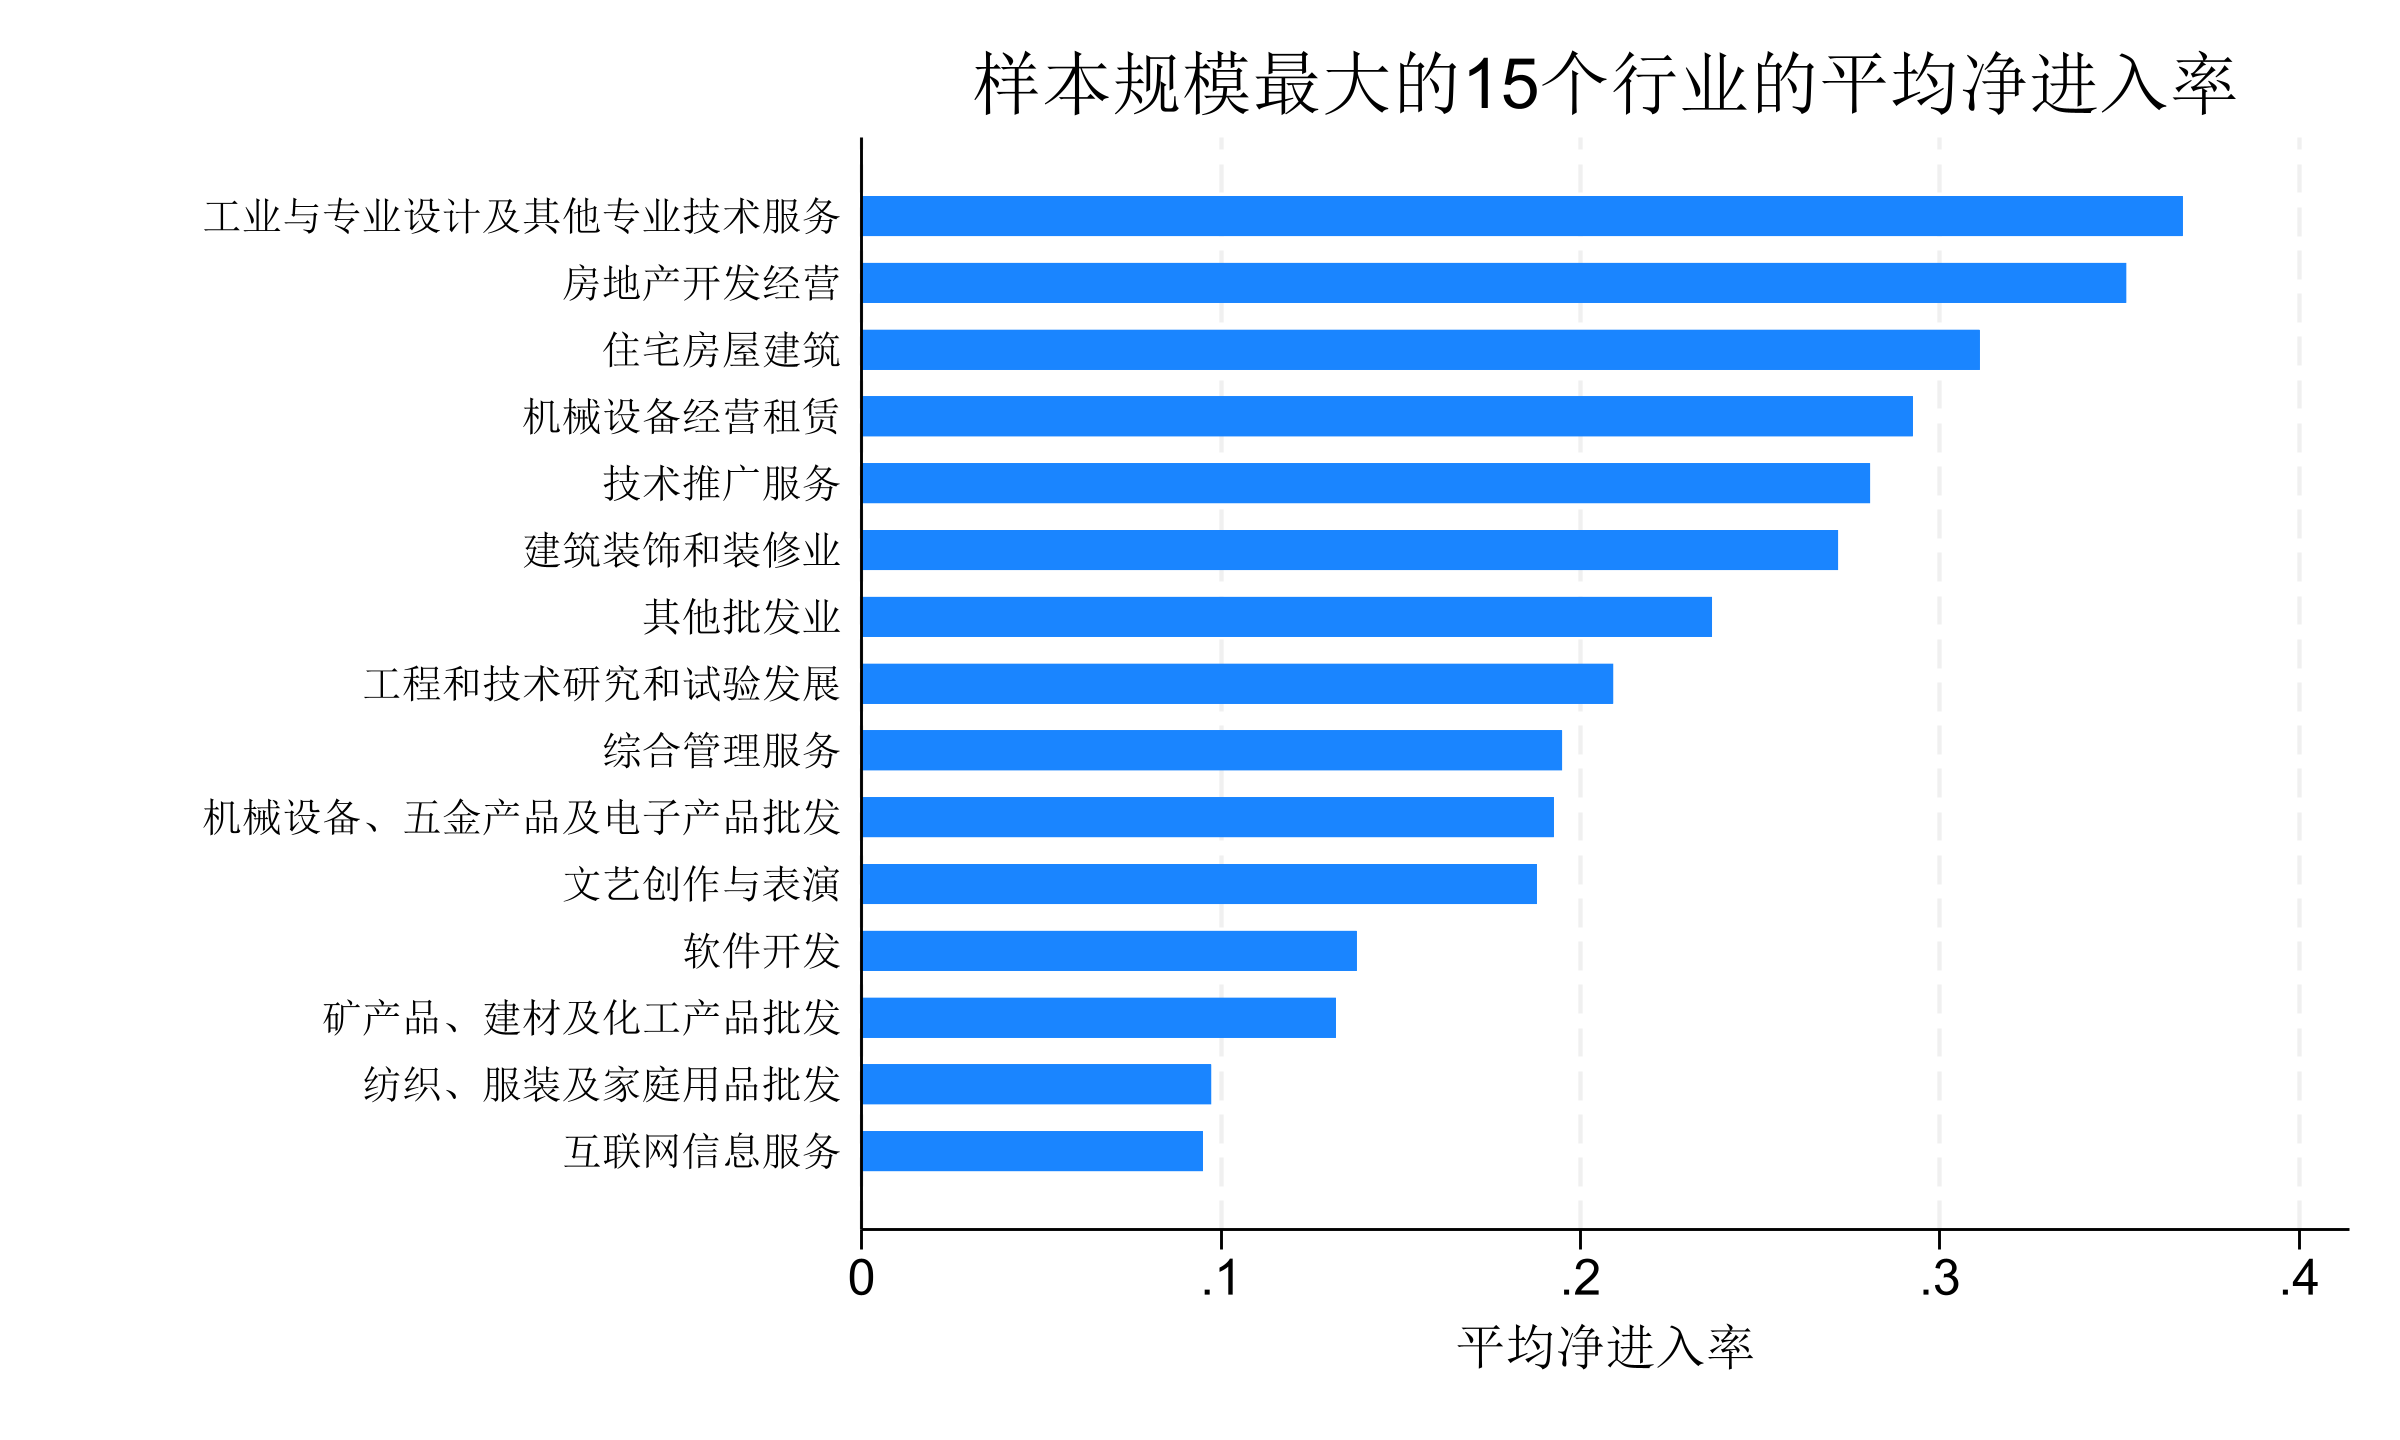
\includegraphics[width=0.92\textwidth]{../output/figures/figure8_industry_net_rate.png}
\caption{样本规模最大的 15 个行业的平均净进入率}
\caption*{\footnotesize 注：横轴无实际数值含义，纵轴为行业名称。柱长表示各行业在样本期内的平均净进入率，仅展示样本规模最大的 15 个行业，用于比较主要行业的净扩张强弱。}
\end{figure}

\begin{figure}[H]
\centering
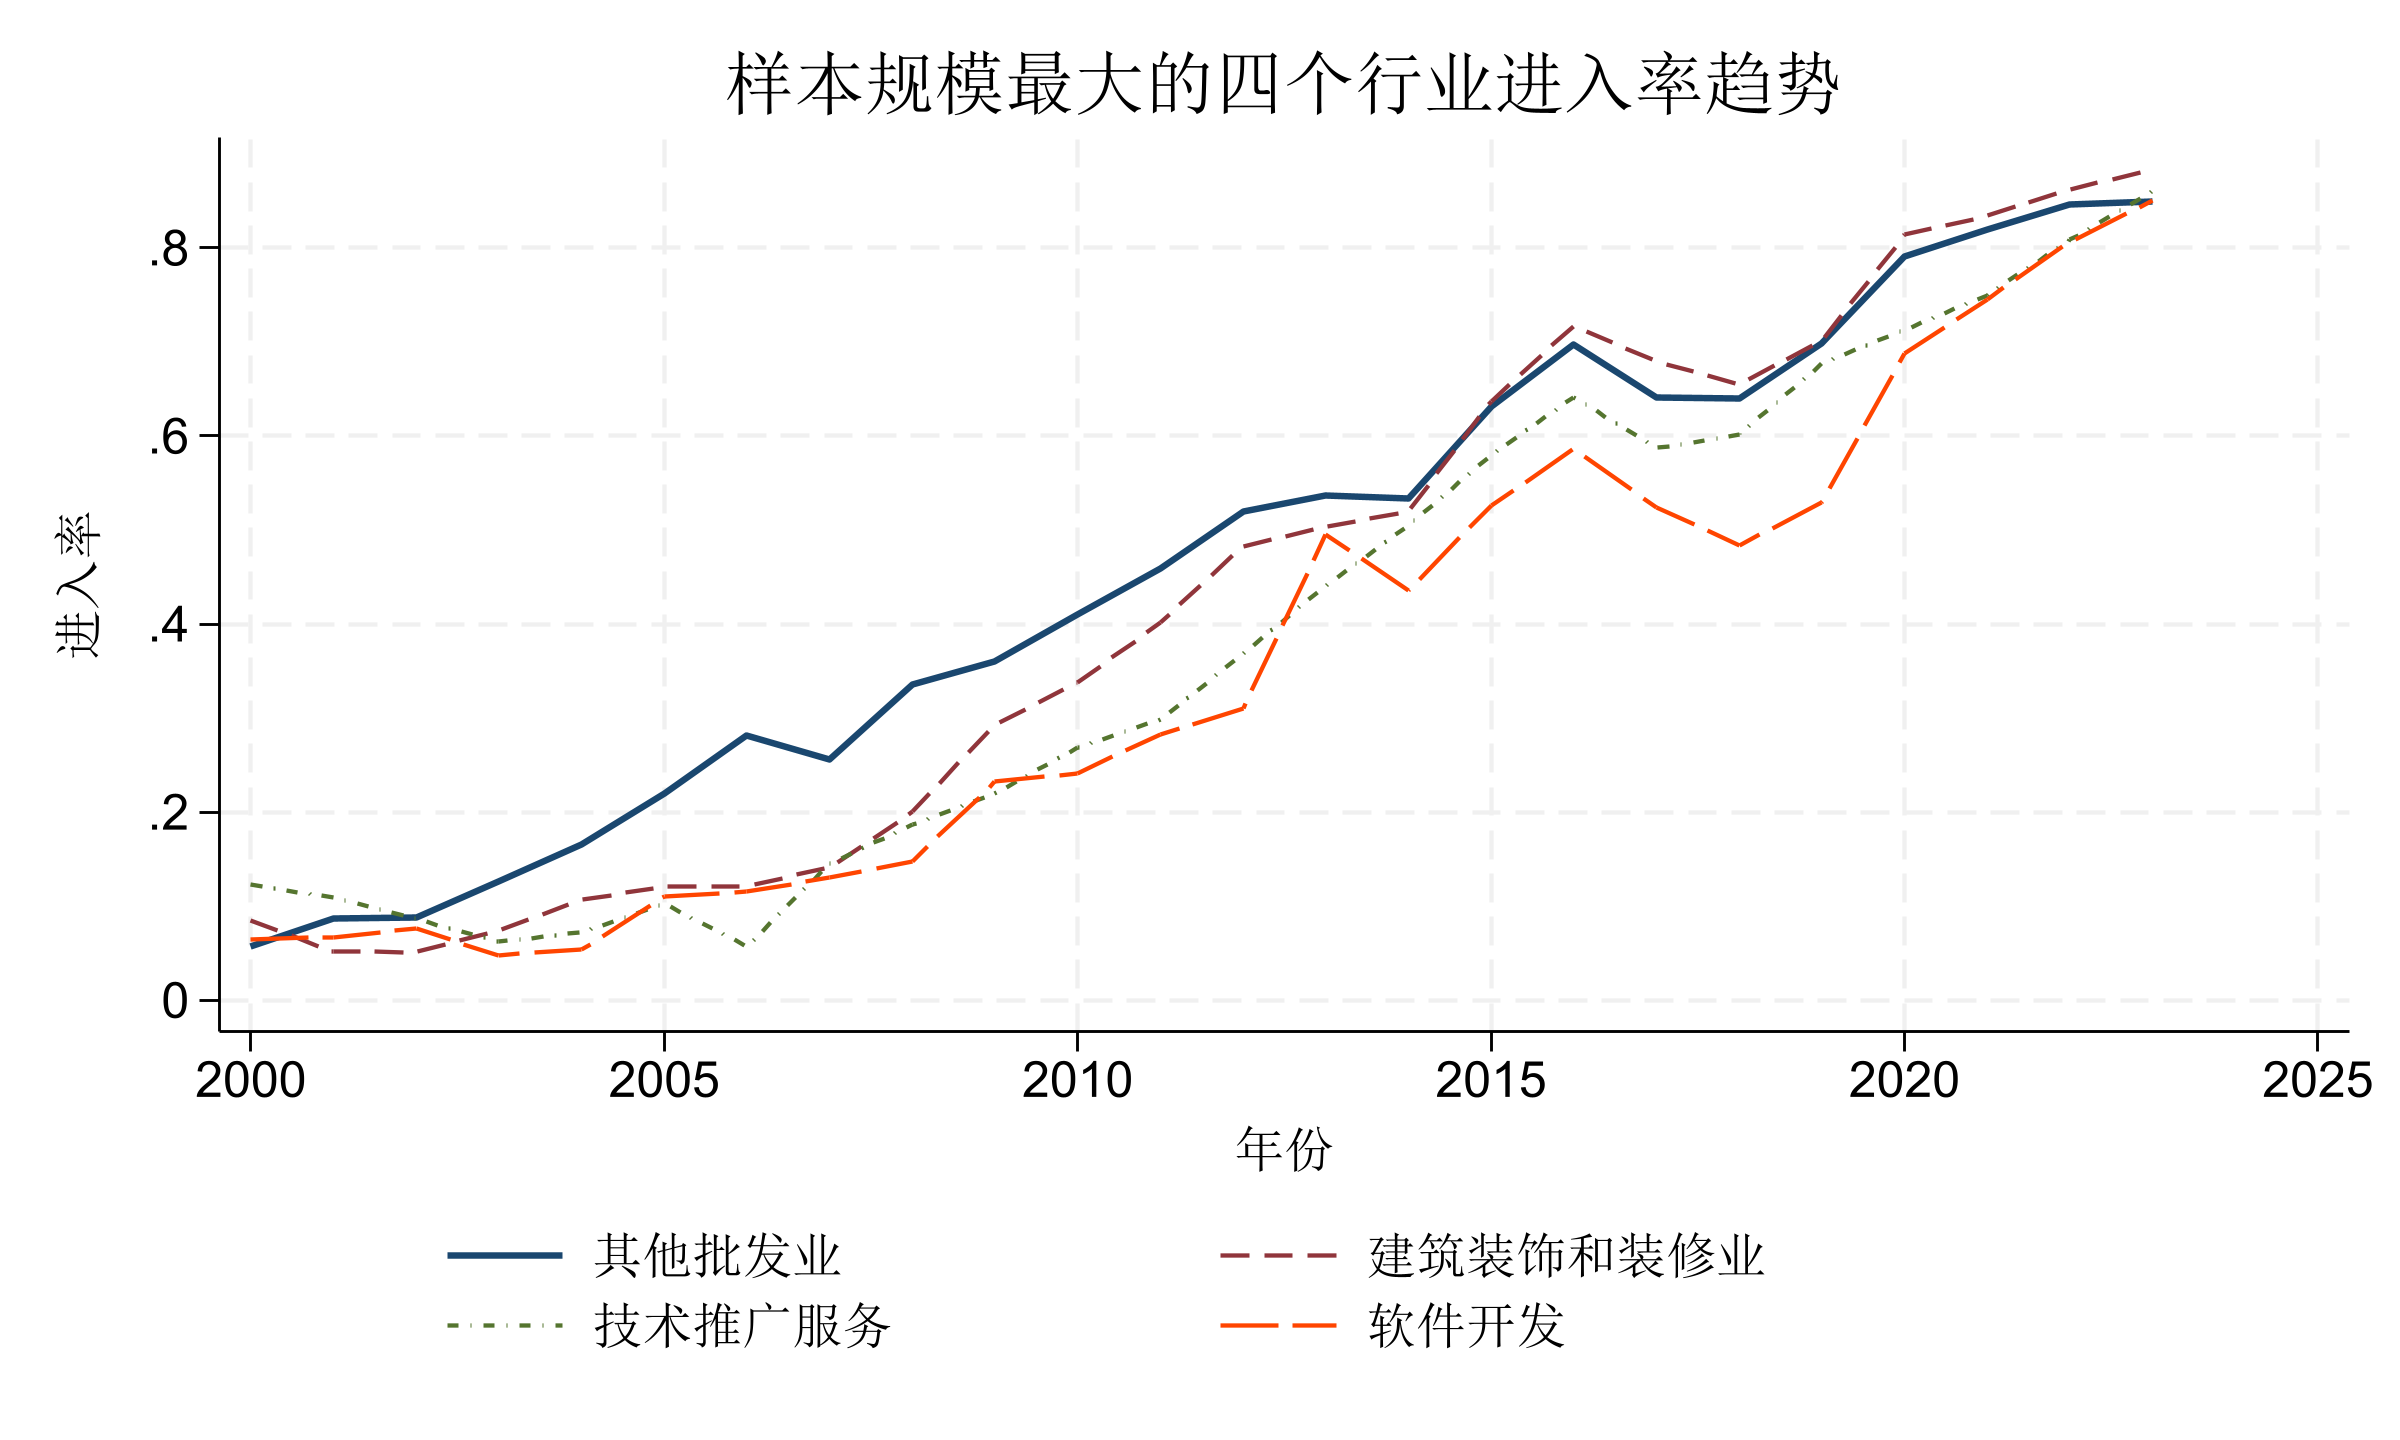
\includegraphics[width=0.92\textwidth]{../output/figures/figure9_industry_entry_trends.png}
\caption{样本规模最大的四个行业进入率趋势}
\caption*{\footnotesize 注：横轴为年份，纵轴为进入率。不同颜色折线分别代表样本规模最大的四个行业，展示这些核心行业吸纳新企业的长期变化路径。}
\end{figure}

\begin{figure}[H]
\centering
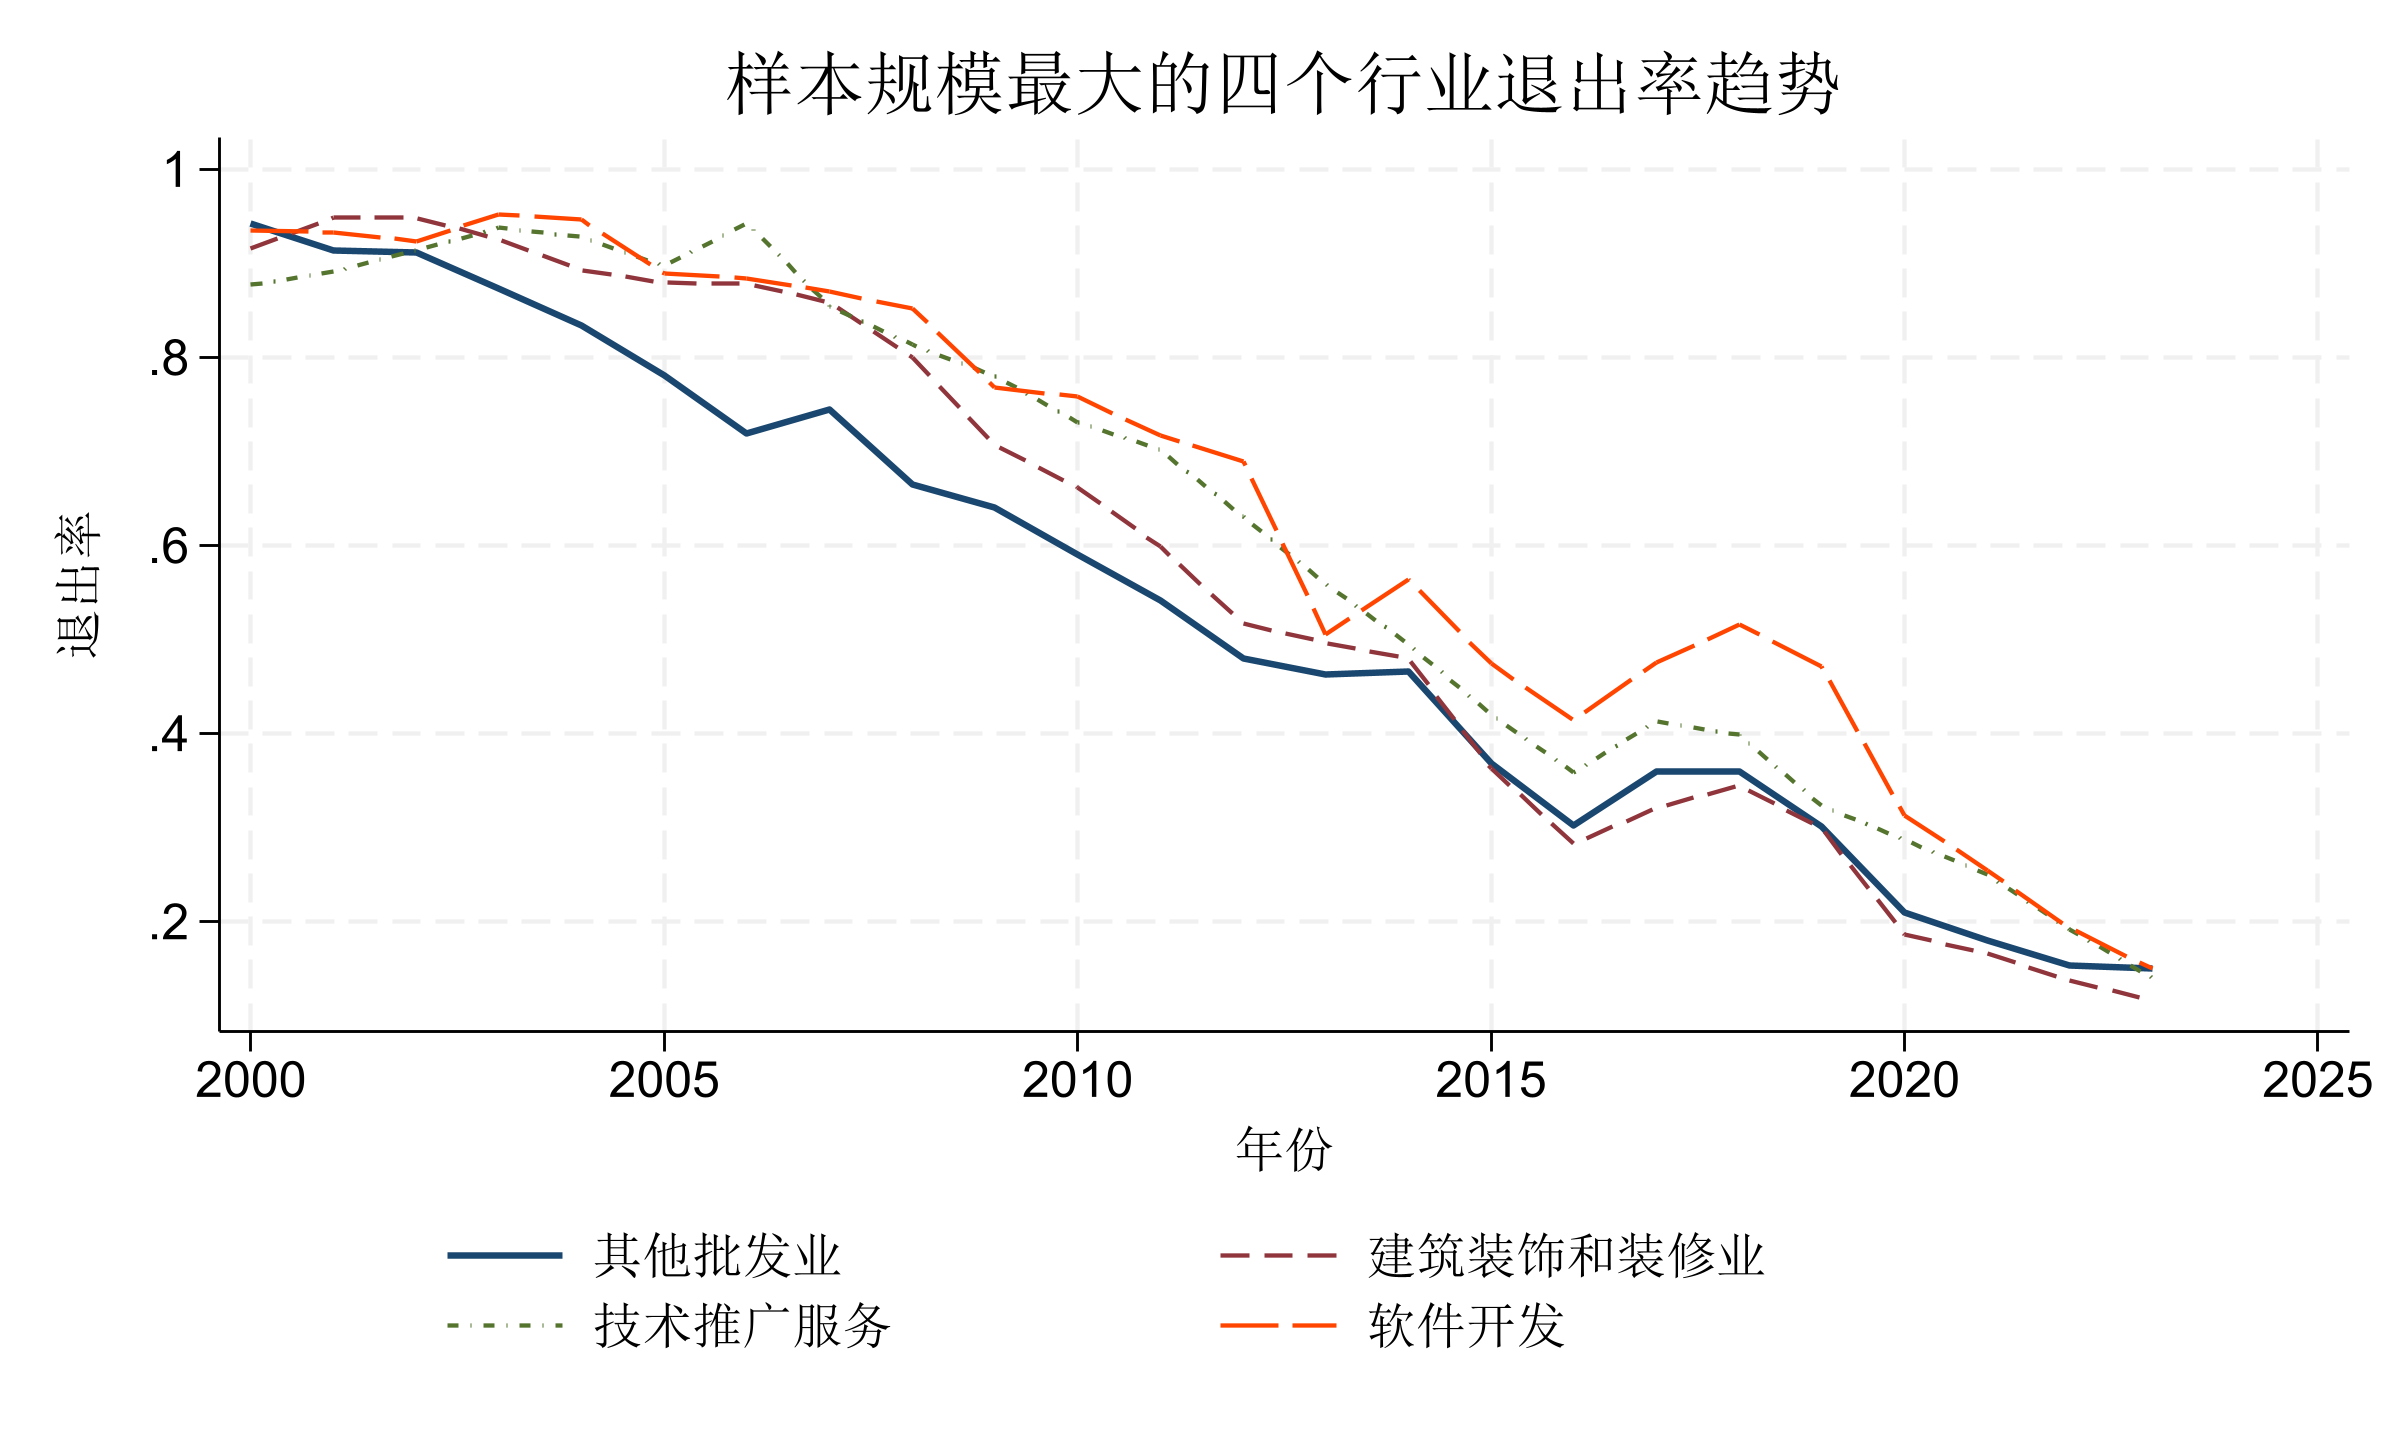
\includegraphics[width=0.92\textwidth]{../output/figures/figure10_industry_exit_trends.png}
\caption{样本规模最大的四个行业退出率趋势}
\caption*{\footnotesize 注：横轴为年份，纵轴为退出率。不同颜色折线分别代表样本规模最大的四个行业，展示这些核心行业的市场出清和企业退出变化。}
\end{figure}

\section{企业生存时间扩展分析}
为了补充进入退出比率之外的动态信息，本文进一步使用新增的企业生存时间数据文件，对不同行业门类企业的平均生存时间进行扩展分析。该扩展数据覆盖 2010--2023 年，共包含 \SurvivalObs\ 个行业--成立年份观测，涉及 \SurvivalIndustries\ 个行业门类。平均来看，样本中的企业生存时间约为 \MeanSurvivalAge\ 年。由于该数据按照行业门类和成立年份汇总，因此它并不直接进入主回归，而是作为对主文企业动态事实的补充说明。这样做的目的，是把“企业进入得多不多”与“企业活得久不久”区分开来，从而补足单纯进入退出比率难以覆盖的另一维度。

图 11 展示了 2015--2020 年不同成立年份企业平均生存时间的相对指数，并统一以 2015 年平均生存时间为基期，将其标准化为 100。这样处理后，cohort 之间的相对变化以及分布上下边界都可以在同一尺度下直接比较。可以看到，随着成立年份向后推进，平均生存时间指数持续下降；与此同时，1\%--99\% 区间带也整体下移且保持可见宽度，说明后续 cohort 的企业生存时间不仅均值下降，其上下尾部分布也同步收缩。换句话说，后期 cohort 面临的并不仅是平均意义上的“更短生存时间”，而是整个分布都在向下移动。

图 12 则更有针对性地比较了行业生存时间溢价。这里的“溢价”定义为某行业在同一成立年份下的平均生存时间，相对于当年全部行业平均值的偏离。结果显示，科学研究和技术服务业、交通运输仓储邮政业以及教育业的生存时间溢价最高，而采矿业、电力热力燃气及水生产供应业以及水利环境公共设施管理业则处于相对较低位置。这说明即便控制成立年份，不同行业的企业耐久性仍存在系统差异，也说明企业生存能力具有鲜明的行业属性。

更有意思的是，企业生存时间与行业净进入率并不呈现简单的正向关系。图 13 将 2010--2023 年各行业门类的平均生存时间与主样本中对应行业大类的平均净进入率放在同一平面上。可以看到，像建筑业这样净进入率很高的行业，并不一定拥有最高的平均生存时间；而科学研究和技术服务业虽然净进入率并非最高，却表现出更高的生存时间溢价。这意味着“新企业大量进入”与“企业存续更久”是两个相关但并不等同的维度，一个城市或行业的营商活力，不能只由净进入率单独刻画。更准确地说，\textbf{营商活力至少同时包含“进入扩张”与“存续质量”两个维度。}

\begin{figure}[H]
\centering
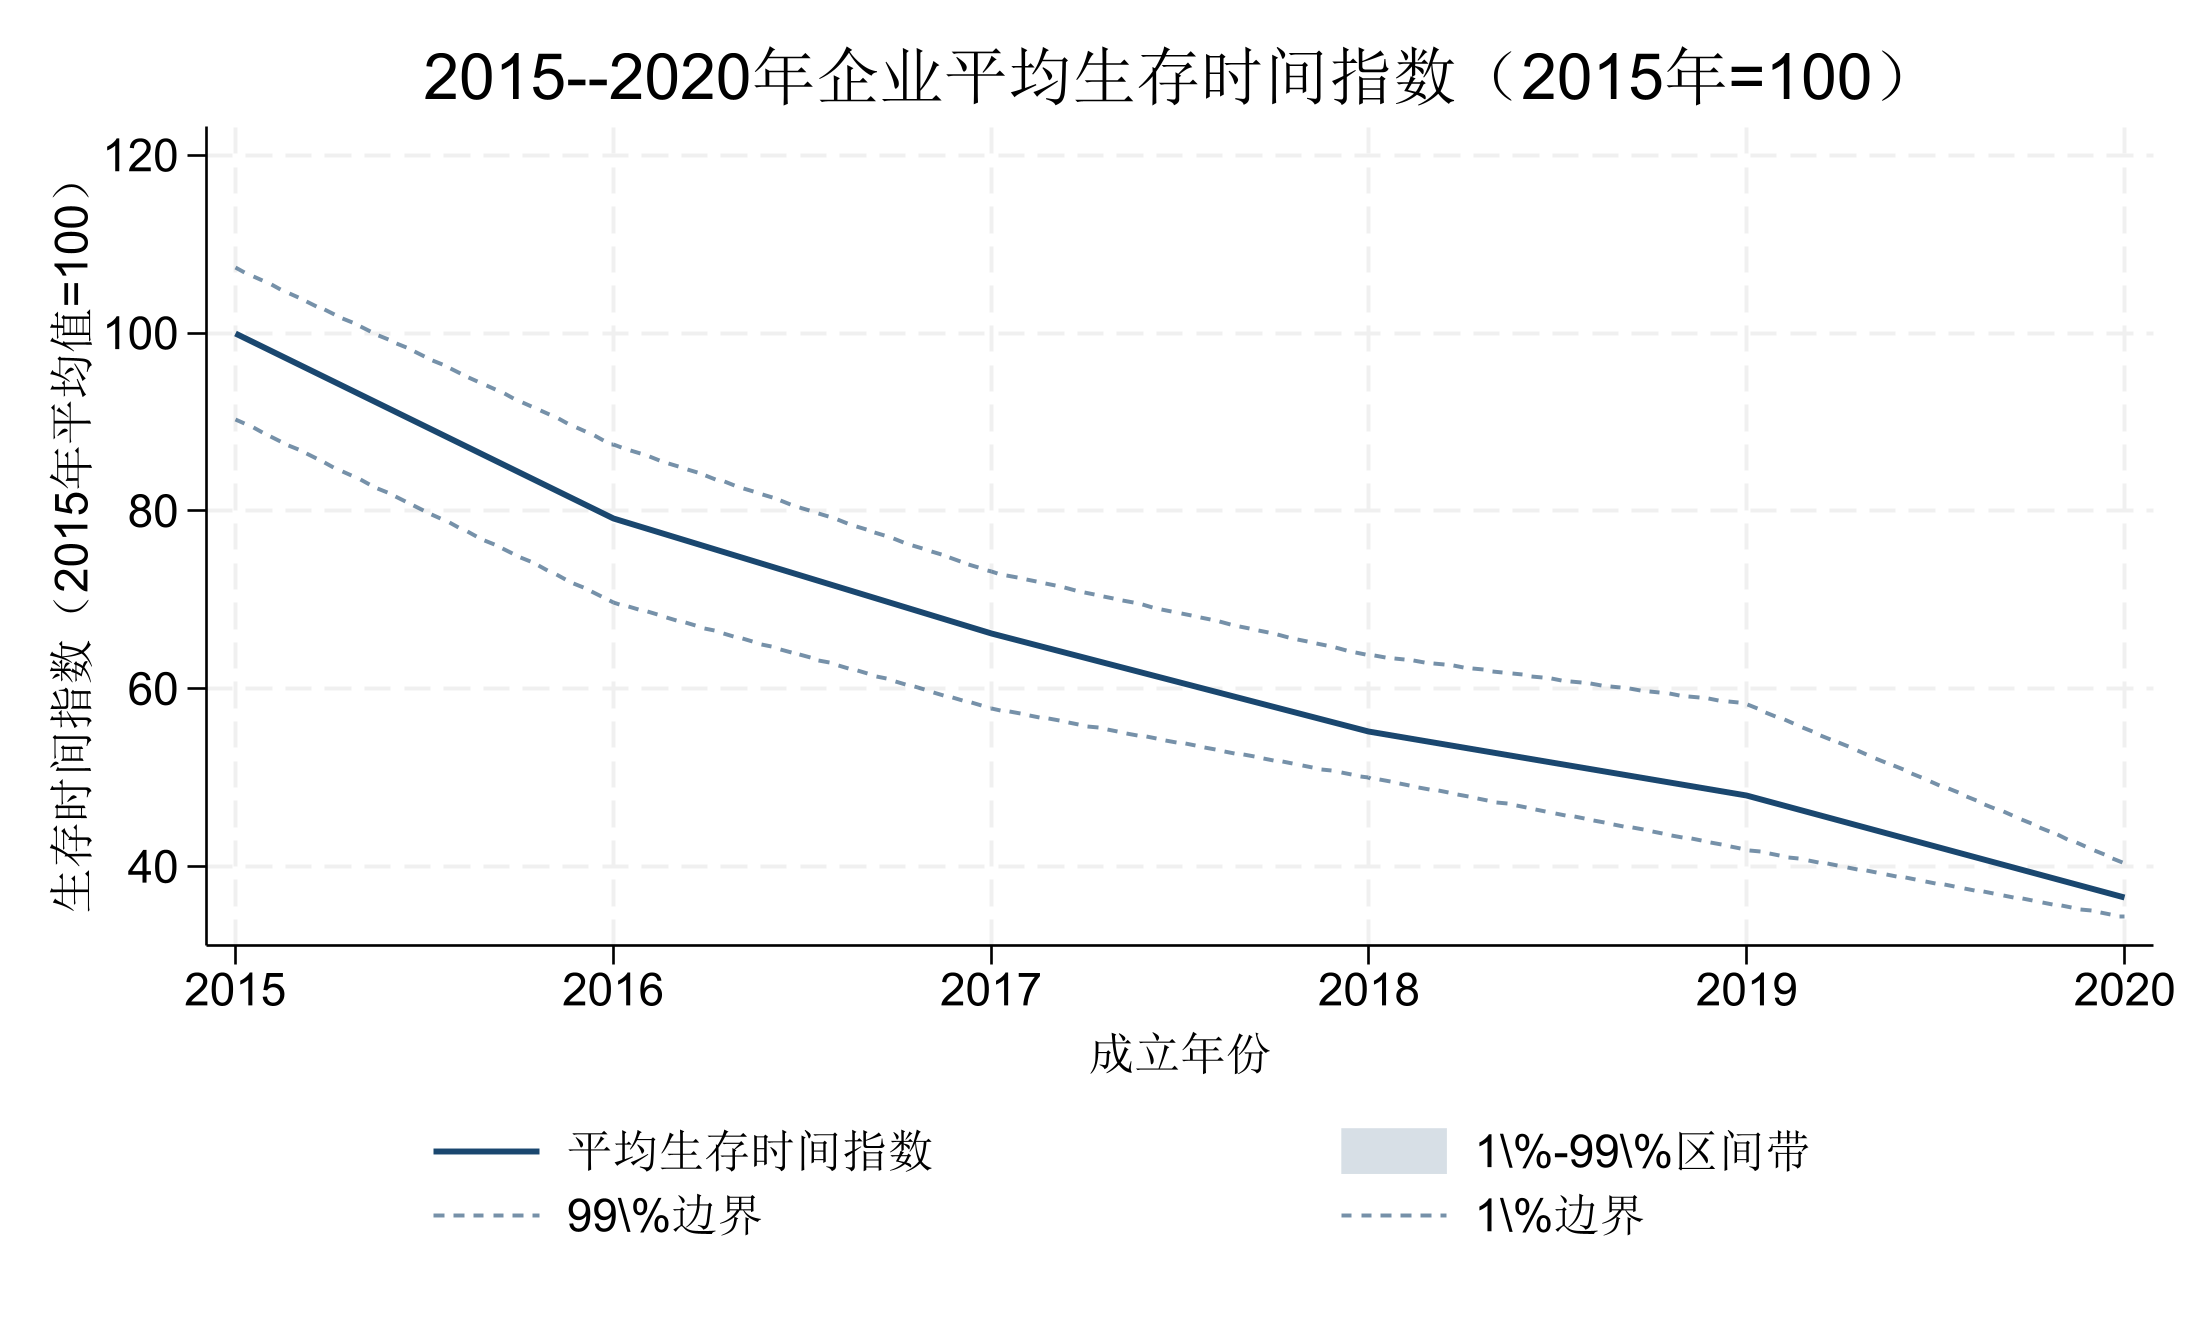
\includegraphics[width=0.9\textwidth]{../output/figures/figure11_survival_cohort_trend.png}
\caption{2015--2020 年企业平均生存时间指数（以 2015 年平均值=100）}
\caption*{\footnotesize 注：横轴为成立年份，纵轴为生存时间指数，并统一以 2015 年平均生存时间为基期标准化为 100。蓝色实线表示各 cohort 的平均生存时间指数；蓝色阴影带表示同一基期下的 1\%--99\% 区间带；两条较浅的虚线分别标示 1\% 和 99\% 边界。由于均值与分位数使用同一基期缩放，因此图中区间带宽度可以直接理解为不同成立年份企业生存时间分布的相对离散程度。}
\end{figure}

\begin{figure}[H]
\centering
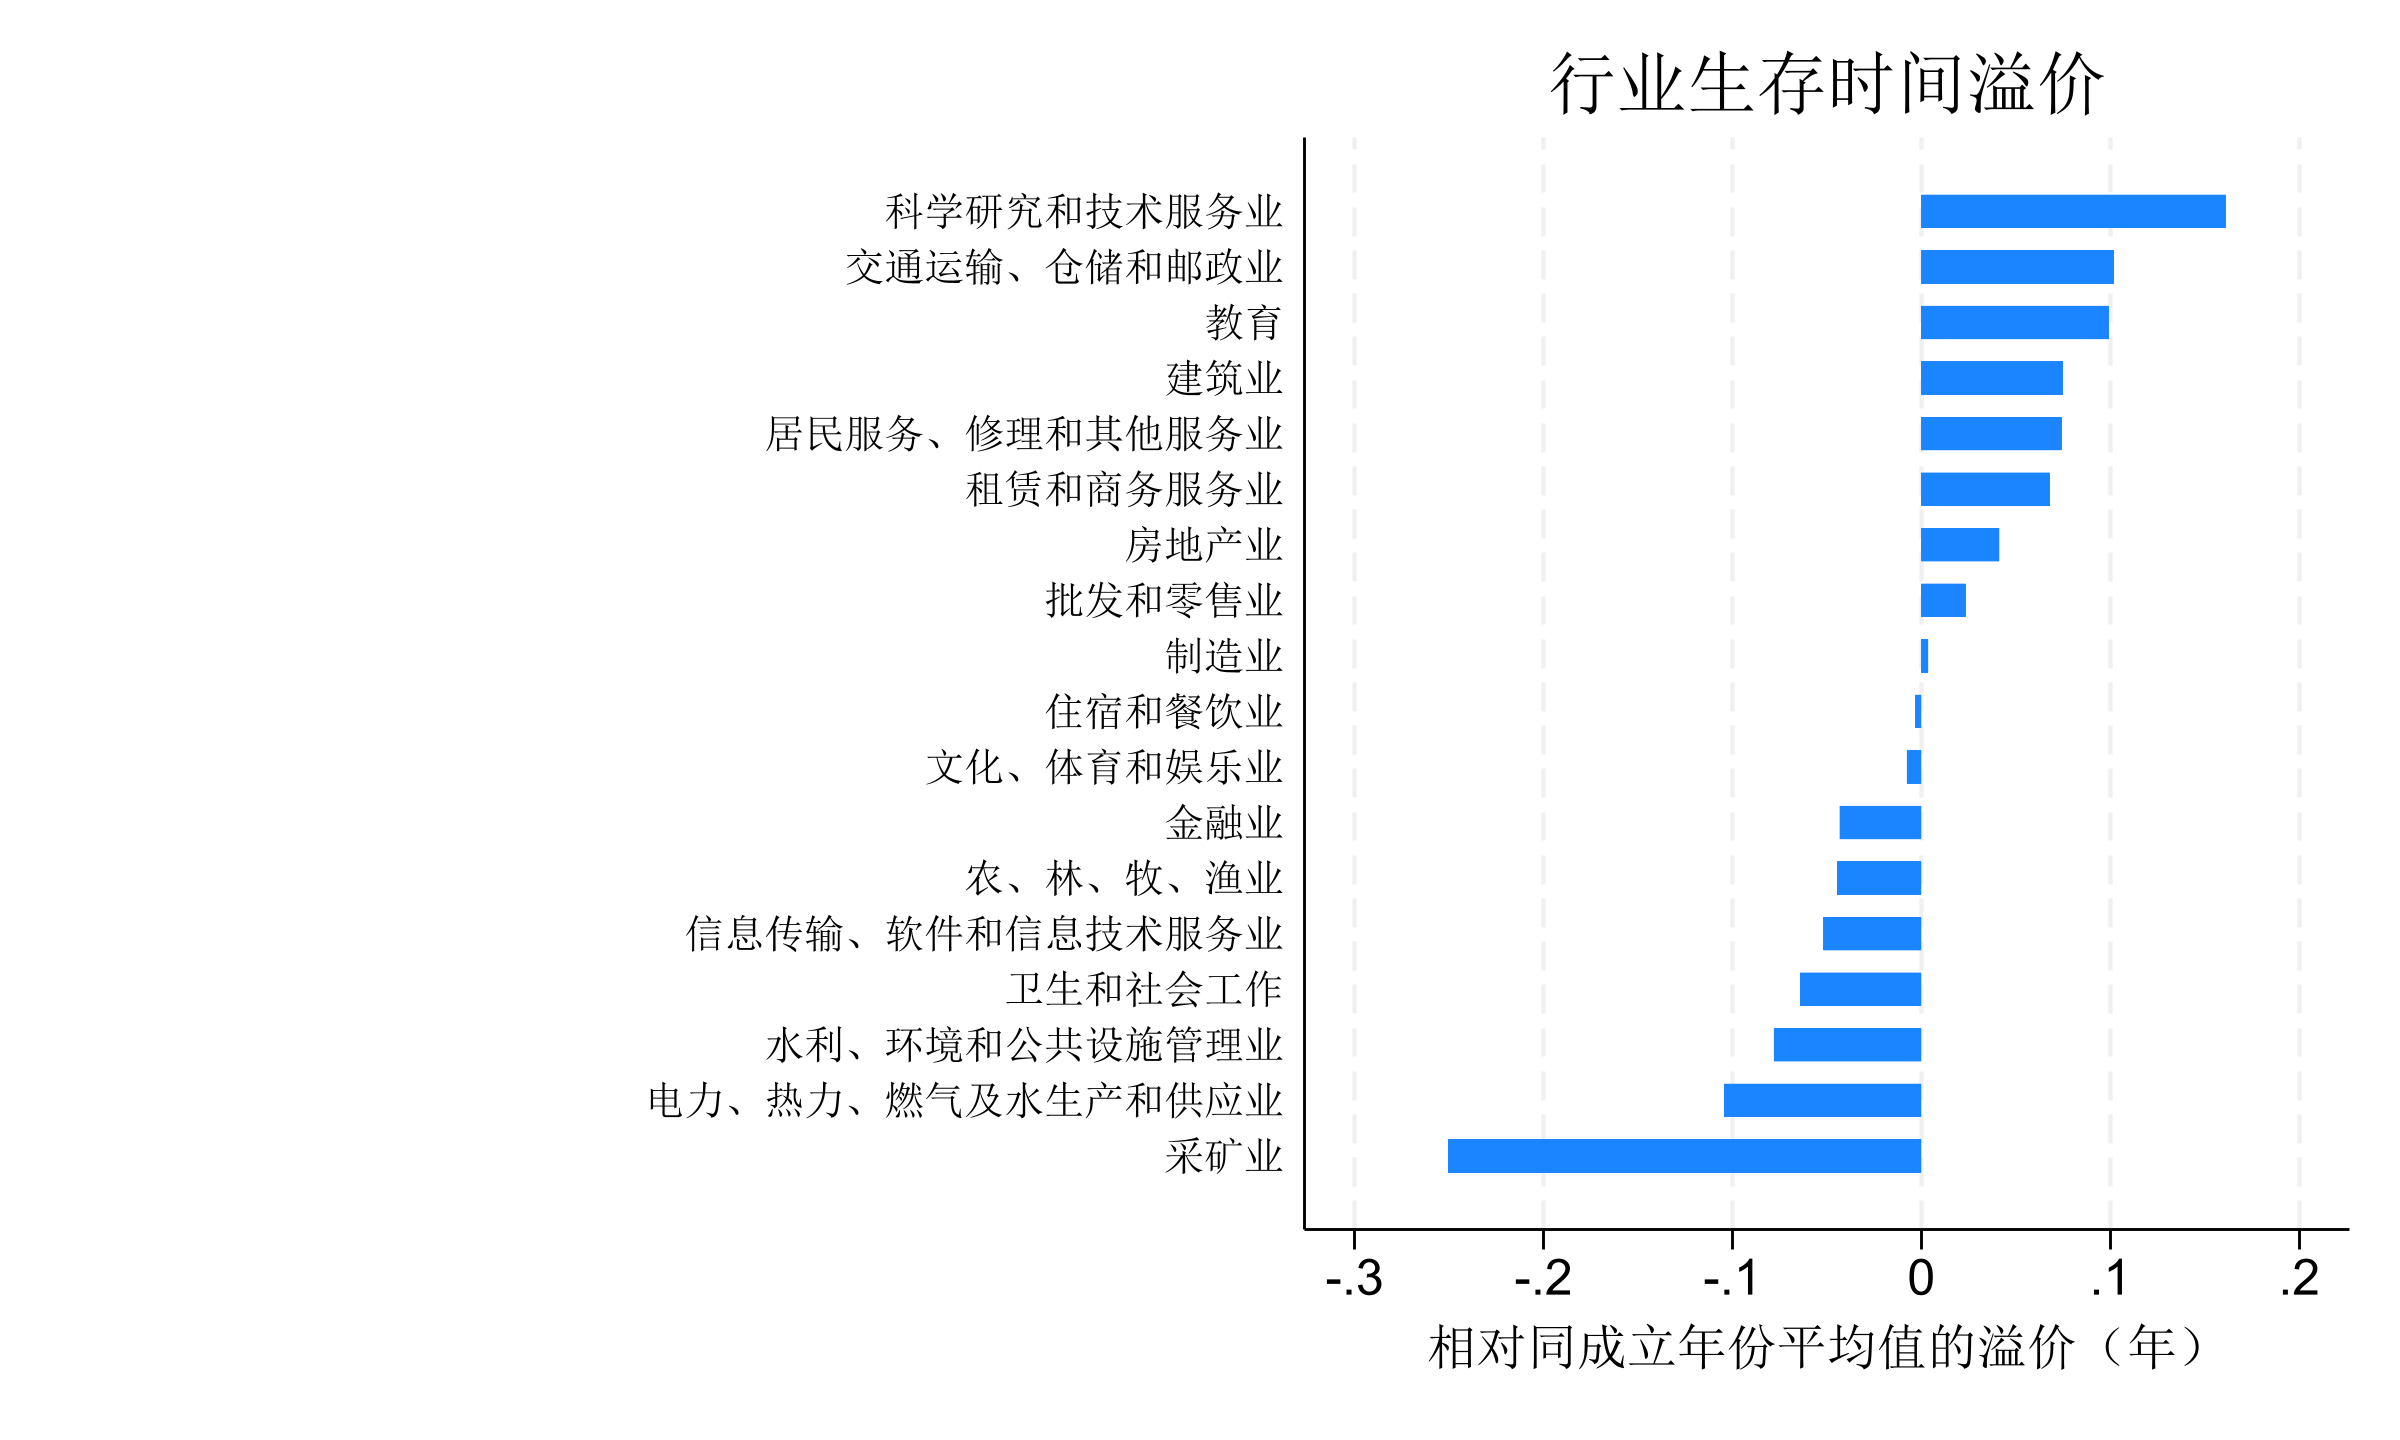
\includegraphics[width=0.92\textwidth]{../output/figures/figure12_survival_premium.png}
\caption{行业生存时间溢价}
\caption*{\footnotesize 注：横轴无实际数值含义，纵轴为行业门类。柱长表示某行业相对于同成立年份全部行业平均生存时间的偏离值，数值越大说明该行业企业平均生存时间越长。}
\end{figure}

\begin{figure}[H]
\centering
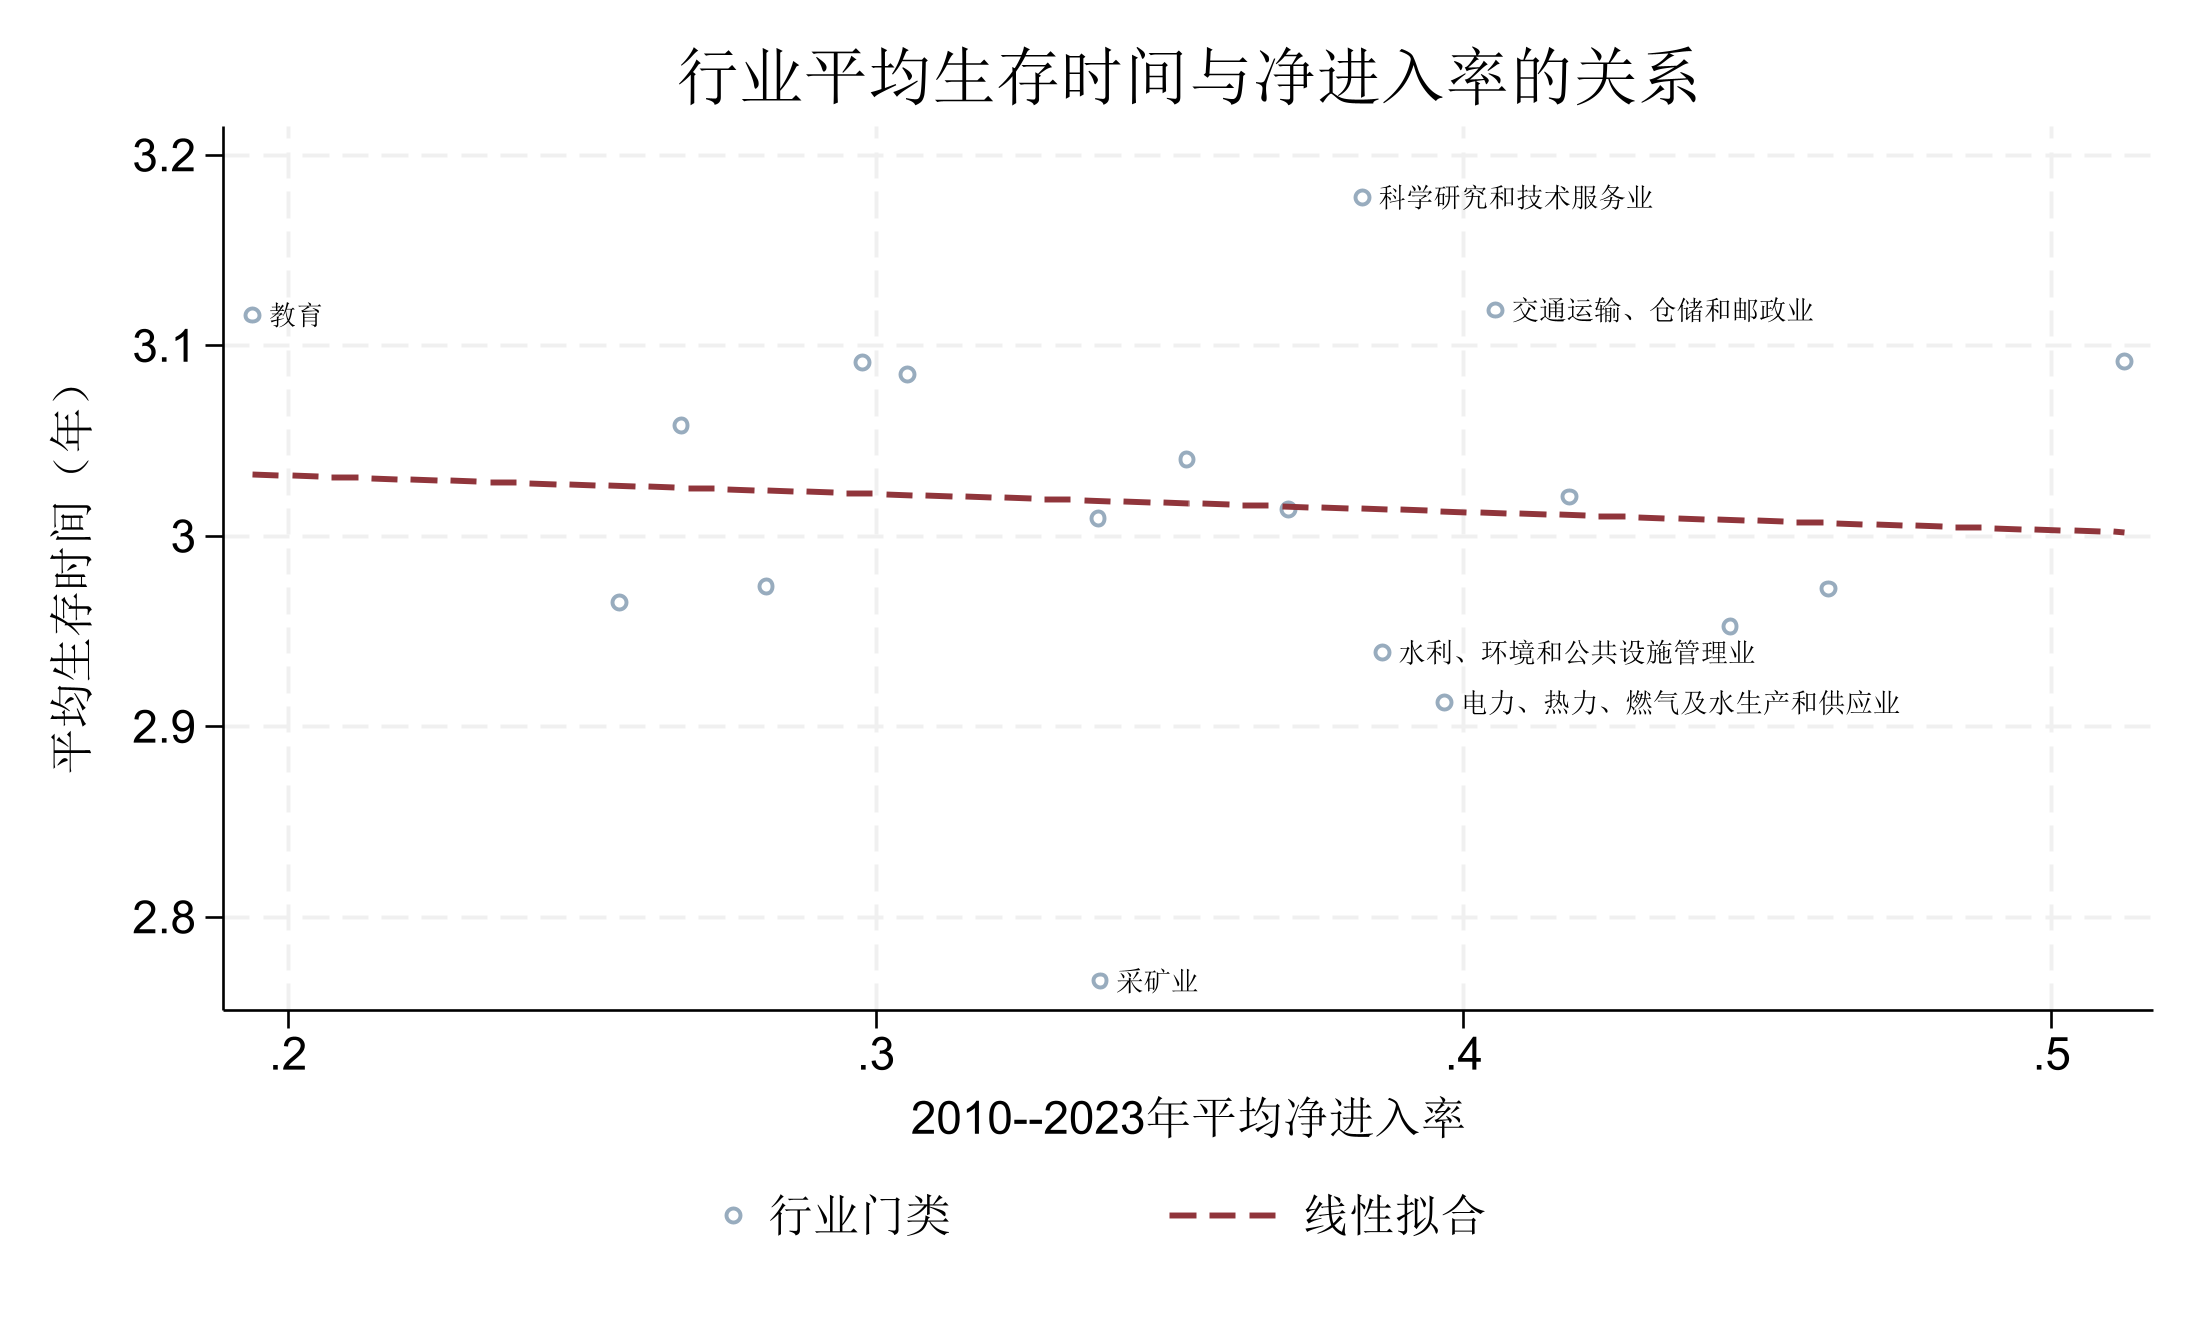
\includegraphics[width=0.88\textwidth]{../output/figures/figure13_survival_netrate_scatter.png}
\caption{行业平均生存时间与净进入率的关系}
\caption*{\footnotesize 注：横轴为 2010--2023 年行业大类的平均净进入率，纵轴为企业平均生存时间。每个圆点代表一个行业门类，圆点大小按主样本中该行业聚合企业总数加权，因此圈子越大表示行业样本规模越大；虚线为线性拟合线，用于描述生存时间与净进入率之间的总体相关方向，部分行业名称被直接标注以突出代表性行业。}
\end{figure}

\section{结论}
本文将主分析口径统一设定为 2000--2023 年全国市级地区--行业--年份面板，并明确要求每个地区--行业--年份单元至少包含 5 条企业记录。在这一统一口径下，本文不仅系统刻画了进入率、退出率和净进入率，还进一步引入城市产业集中度 HHI，并在扩展部分加入企业生存时间分析，将企业动态与产业结构结合起来考察。全文的核心思路可以概括为：先在统一口径下识别城市行业单元的进入退出事实，再把这种事实放回城市产业结构和企业存续维度中重新理解。

结果表明，第一，样本期内企业进入总体上显著高于退出，行业单元层面长期呈现净进入格局。第二，城市产业集中度 HHI 呈明显下降趋势，说明随着行业单元扩张，城市产业结构整体趋于多元化。第三，企业进入退出具有显著持续性，而行业单元规模与后续净进入率之间在总体上表现为负相关，但这一关系在东部和副省级城市中明显减弱。第四，行业异质性非常突出，大规模服务业、技术类和批发类行业共同构成了当前城市企业动态的核心板块。第五，从扩展分析看，不同行业存在清晰的生存时间溢价，而净进入率较高并不必然意味着企业生存时间更长。综合而言，\textbf{中国城市营商活力并不是单一指标上的扩张，而是净进入、产业多元化与企业存续质量共同作用的结果。}

未来若要进一步深化研究，可以继续在保持同一统计层次的前提下，引入 GDP、财政、人口、创新政策或营商环境评估指标，解释为什么某些城市能够同时实现较低集中度和较高净进入率；也可以基于本文已经构建的 HHI 指标，进一步分析产业多元化与企业存活、城市韧性之间的关系。无论如何，\textbf{统一统计口径}仍然是后续研究获得清晰解释的前提，也是本文最希望强调的方法论出发点。

\end{document}
